\PassOptionsToPackage{unicode}{hyperref}
\PassOptionsToPackage{hyphens}{url}
%
\documentclass[12pt, a4paper]{article}
\usepackage[a4paper,margin=3cm]{geometry}
\setlength\parindent{0pt}
\usepackage{mathptmx}
\usepackage{amsmath,amssymb}
\usepackage[T1]{fontenc}
\usepackage[utf8]{inputenc}
\usepackage{textcomp}
\usepackage{graphicx}
\usepackage{float}
\usepackage{booktabs}
\usepackage[justification=centering]{caption}
\usepackage{hyperref}

% NOTE: course rules require groups of 3-5 students; list every member as
% "Name Surname, Degree Programme, ID number (matricola)" per the official template.
\author{Pietro Tellarini\\ Master's Degree in Artificial Intelligence, 0001145761 \\
Kawsar Farooq\\ Master's Degree in Artificial Intelligence, 0001157200}
\date{}
\title{Network Analysis of the Bologna Transit System: Bottlenecks and Resilience}


\begin{document}
\maketitle

\section{Introduction}
\label{introduction}

The emergence of Network Science and Social Network Analysis (SNA) has provided a robust mathematical lexicon and statistical apparatus for studying complex socio-tech\-ni\-cal systems~\cite{newman}. Rather than viewing infrastructures as isolated physical entities, Network Science allows us to abstract and model them as topological graphs in which entities are nodes and their relations are edges. Although originally developed for social and biological systems, this structural paradigm has become increasingly important in urban planning, transport geography, and infrastructure engineering, where it enables the quantitative study of how spatial configurations influence human mobility, municipal accessibility, and system-wide vulnerability.

This project examines the topological structure of the public transit network of Bologna, Italy. Developed within the Master's Degree in Artificial Intelligence at the University of Bologna, the study investigates the structural transition of Bologna's mobility system. Historically reliant on a radial bus network, Bologna is currently implementing a new tram system (including the new Red and Green lines) intended to serve as the high-capacity backbone of its urban core.

Our analysis models these transit layers as complex spatial networks across a structured narrative:
\begin{itemize}
    \item \textbf{Data and Methodology (Baseline Setup)}: GTFS and OpenStreetMap data cleaning, mapping of municipal population statistics to stations, and construction of L-space and P-space topologies weighted by traffic congestion and population pressure.
    \item \textbf{Classical Baseline Transit Study}: Analysis of cognitive P-space communities, physical L-space bottlenecks, macroscopic small-world indices, and resilience under random and targeted failures for the Bus Only and Planned Tram networks.
    \item \textbf{Future Scenarios Exploration}: Two predictive scenarios: upgrading the circular ring-road Lines 32/33 into a fast tramway, and designing an optimal tramway from scratch with a multi-criteria greedy algorithm.
    \item \textbf{Commuter Shock Analysis}: Stress-testing all four networks under massive commuter injections at the central station hubs to compare local shock absorption.
\end{itemize}

In total, the study analyzes \textbf{six networks}: four L-space graphs (Bus Only, Planned Tram, Circular Tram, Optimal Tram) and two P-space graphs (Bus Only, Planned Tram). All six are \textbf{monomodal (unipartite), undirected} graphs whose nodes are physical transit stops. L-space edges connect consecutive stops along a service line and are \textbf{weighted} by travel time in seconds; P-space edges connect any two stops sharing at least one line and are \textbf{unweighted}.

\section{Problem and Motivation}
\label{problem-and-motivation}

Urban transit networks are subject to two opposing engineering and geographical pressures: the necessity for high routing efficiency and the requirement for structural resilience against localized failures. Traditional radial bus networks, which converge heavily on a few historical centre-city corridors, are notoriously vulnerable to traffic congestion and localized disruptions: a single street blockage can cascade delays across dozens of lines.

To address these challenges, we analyze the transit system across four configurations:
\begin{enumerate}
    \item \textbf{Bus Only}: The baseline radial bus infrastructure.
    \item \textbf{Planned Tram}: An integrated model of the planned tram lines (Red and Green), where nearby bus and tram stops are merged into single nodes if they fall within a topological snapping radius of $30\text{ m}$ (representing the physical proximity of shared platform bays).
    \item \textbf{Circular Tram}: A predictive scenario upgrading the circular ring-road bus Line 32 (clockwise) and Line 33 (counter-clockwise) into a fast, dedicated tramway in addition to the planned tramways, evaluated to determine its capacity to mitigate central bottleneck pressure.
    \item \textbf{Optimal Tram}: An algorithmically designed tramway network built from scratch under a fixed spatial budget to maximize accessibility.
\end{enumerate}

Our research design relies on key literature in complex networks:
\begin{itemize}
    \item \textbf{Small-World Efficiency}: Latora and Marchiori~\cite{latora2} demonstrated in their study of the Boston subway that transportation networks, despite being constrained by two-dimensional physical space (spatial planarity), can still exhibit small-world characteristics. They introduced ``global efficiency'' as a metric of how efficiently a network forwards information or passengers, which we adopt to measure travel-time utility.
    \item \textbf{Robustness under Attack}: Derrible and Kennedy~\cite{derrible} analyzed 33 metro systems globally, showing that transit networks are often scale-free-like structures dominated by major transfer hubs. This topology exhibits high resistance to random failures but extreme fragility under targeted attacks.
\end{itemize}

The main contribution of this project is a data-driven, reproducible analysis pipeline for Bologna. The complete source code and generated datasets are open source and available on GitHub in the \href{https://github.com/PtrTella/UrbanNetwork/tree/feature/bologna-transit-analysis}{\texttt{feature/bologna-transit-analysis}} branch. It models traffic congestion via the Bureau of Public Roads (BPR) function, maps municipal population data onto the network, and simulates structural percolation.

\section{Datasets}
\label{datasets}

The data was compiled from multiple open municipal and open-source datasets to ensure reproducibility:
\begin{enumerate}
    \item \textbf{GTFS (General Transit Feed Specification)}: Obtained from TPER (Trasporto Passeggeri Emilia-Romagna), the regional transport operator. The feed was filtered through a curated white-list of urban routes, so that the resulting graph represents the urban bus network of Bologna (radial, tangential, and city-centre shuttle lines).
    \item \textbf{OpenStreetMap (OSM)}: Tram stop locations (existing, under construction, and proposed) were extracted via the Overpass API using a custom script. The stop sequences and branch topology of the new tram routes (Line 1/Rossa and Line 2/Verde) were curated in a structured JSON file and geocoded against the OSM extract, with fallbacks on GTFS bus-stop coordinates and the Nominatim geocoder.
    \item \textbf{Traffic Spire Flows}: Sourced from the Open Data portal of the Municipality of Bologna, capturing vehicle counts measured by induction-loop detectors in 2026.
    \item \textbf{Accidents Dataset}: Municipal registry of road accidents, used to compute a localized risk index within a 300-metre buffer of each bus stop.
    \item \textbf{Resident Population Statistics (2024)}: Neighbourhood-level resident populations published by the Municipality of Bologna, aggregated by statistical area.
\end{enumerate}

We used the Python library \texttt{GeoPandas} for spatial data processing (including geographic buffers and nearest-neighbour spatial joins), \texttt{NetworkX} as the core mathematical engine to construct and analyze the network topologies, and \texttt{scikit-learn} for spatial clustering (DBSCAN) of stops into urban macro-zones. The final visualizations were generated with \texttt{Matplotlib} and \texttt{Seaborn} (static reporting graphs) and \texttt{Folium} (interactive HTML maps).

\section{Validity and Reliability}
\label{validity-and-reliability}

To guarantee the \textbf{validity} of our model (how closely it mirrors the real physical system), we developed a hybrid network--physical framework. Rather than restricting the study to a purely topological analysis, we overlaid a geographical and transportation-engineering engine implementing the following core components.

\subsection{L-space vs. P-space Representation}
In transit network analysis, networks can be modeled in L-space (nodes represent physical stops, edges denote consecutive adjacent service hops) or P-space (edges connect any two stops sharing a transit line). We selected L-space as the primary representation because it preserves the physical layout of roads and rails. This is a prerequisite for studying infrastructural vulnerability, localized road congestion, and detour routing~\cite{derrible}. The P-space representation is used in Act~1 to study transfer-free travel and community structure.

\subsection{BPR Congestion Weights (Supply Friction)}
Instead of static geographical distances, edges are weighted by travel times (in seconds):
$$t_{travel} = \frac{d}{v_{effective}} + t_{base\_dwell}$$
where $t_{base\_dwell}$ is the baseline vehicle dwell time ($5.0\text{ s}$ for buses, $8.0\text{ s}$ for trams). The effective speed $v_{effective}$ is modeled with the standard Bureau of Public Roads (BPR) congestion function, widely adopted in transit speed impedance modeling and multi-modal traffic assignment~\cite{ryu, pi}:
$$v_{effective} = \frac{v_{base}}{1 + \alpha_{bus} \left( \frac{V + PCU_{bus}}{C} \right)^\beta}$$
where $v_{base}$ is the commercial base speed ($15.0\text{ km/h}$, i.e.\ $4.16\text{ m/s}$, for buses; $20.0\text{ km/h}$, i.e.\ $5.5\text{ m/s}$, for trams, which run on protected right-of-way and are therefore exempt from the congestion term), $V$ is the hourly traffic volume from municipal loop detectors, and $C$ is the road capacity. Crucially, rather than using a uniform value, $C$ is estimated for each segment from the nearest loop detector, defined as $110\%$ of the absolute historical peak flow observed by that sensor (clamped to a minimum of $300\text{ veh/h}$ to avoid mathematical anomalies on minor streets). Segments without usable detector data fall back to a standard urban lane capacity of $800\text{ veh/h}$. The coefficient $\alpha_{bus}=0.20$ and exponent $\beta=4.0$ are standard BPR congestion parameters, and $PCU_{bus} = 2.5$ is the Passenger Car Unit equivalent representing the road occupancy of a standard bus. To prevent total gridlock in the model, the effective speed is clamped to a minimum commercial speed of $1.0\text{ m/s}$ ($3.6\text{ km/h}$), representing crawl speed under total congestion.

\subsection{Demographic Snapping \& Baseline Passenger Pressure}
To realistically represent passenger demand, neighbourhood-level resident population data (2024 municipal statistics) were mapped to physical transit stops. Because GTFS stop names and the municipal stop registry do not match perfectly, we implemented a hybrid matching algorithm with a pedestrian catchment radius of $400\text{ m}$ (roughly a 5-minute walk). The population of each statistical area is divided equally among the stops located within it, and the resulting per-stop weights are assigned as follows:
\begin{enumerate}
    \item Stops with an exact (normalized) name match in the municipal stop registry are associated directly.
    \item Unmatched stops are snapped to the nearest georeferenced stop record with a known statistical area, within a maximum radius of $400\text{ m}$.
    \item Extra-urban stops, and stops beyond the catchment limit, are assigned a zero baseline value.
\end{enumerate}

Running this snapping pipeline on the integrated Planned Tram network (1,283 stops) produced the following results:
\begin{itemize}
    \item \textbf{Exact matches by name}: 1,017 stops.
    \item \textbf{Spatial snaps (catchment buffer $\le 400\text{ m}$)}: 65 stops.
    \item \textbf{Unassociated/extra-urban stops}: 201 stops.
\end{itemize}

Table~\ref{tab:top_pop_stops} lists the five stops with the highest demographic passenger pressure. Note that ranks 2--5 are tied: these stops belong to the same statistical area (Borgo Panigale), whose population is divided equally among its stops.

\begin{table}[H]
    \centering
    \caption{Top 5 Transit Stops by Snapped Demographic Population}
    \label{tab:top_pop_stops}
    \begin{tabular}{clc}
        \toprule
        Rank & Stop Name & \shortstack{Snapped Population\\(Residents)} \\
        \midrule
        1 & SAN DONNINO & 2,922 \\
        2 & SCALA & 1,583 \\
        3 & CHIESA BORGO PANIGALE & 1,583 \\
        4 & BORGO PANIGALE - MUSEO DUCATI & 1,583 \\
        5 & BORGO PANIGALE CIMITERO & 1,583 \\
        \bottomrule
    \end{tabular}
\end{table}

This demographic pressure directly scales the station dwell times: each edge inherits an additional boarding-time penalty proportional to the population served by its downstream stop, so high-population stops dynamically inflate travel times on their incident edges:
$$t_{dwell} = t_{base\_dwell} + \frac{P_{stop} \cdot \theta}{F_{capacity}}$$
where $t_{base\_dwell}$ is $5.0\text{ s}$ for buses and $8.0\text{ s}$ for trams, $\theta = 0.015\text{ s/capita}$ is the marginal boarding time per potential passenger, and $F_{capacity}$ is a door-capacity boarding factor ($1.0$ for buses, $3.0$ for trams). The factor $F_{capacity} = 3.0$ reflects the boarding-speed advantage of modern trams: while a standard bus has 2--3 narrow doors with steps, a tram offers 4--6 wide double-doors and full low-floor level boarding, allowing roughly three times faster passenger exchange. This formulation links physical network topology directly to urban demographic demand, in line with recent empirical evidence that node importance correlates strongly with passenger demand in urban public transport systems~\cite{sfiligoj}, and allows us to evaluate bottlenecks under realistic pressure.

\subsection{Modeling Assumptions and Symmetries}
Several simplifying modeling assumptions were adopted for tractability:
\begin{itemize}
    \item \textbf{Undirected Graph Symmetry}: The network is modeled as an undirected graph (\texttt{nx.Graph}) to allow the calculation of standard global efficiency metrics. In reality, passenger flows can be asymmetric, and transit systems are increasingly modeled as multiplex or multilayer graphs to capture modal switches and transfers~\cite{dedomenico}.
    \item \textbf{Unified Bus-Lane Congestion}: BPR congestion is applied on the basis of overall road capacity, representing corridors where bus lanes merge with general traffic.
    \item \textbf{Dynamic Targeted Attacks}: In real-world failures, traffic redistributes dynamically. We therefore implemented a \textbf{dynamic (sequential) targeted attack} in which betweenness centrality is recalculated after every node removal~\cite{albert}, in addition to the static-ranking percolation analysis.
    \item \textbf{Omitted Measures}: We omit the triad census, which is designed for directed networks; in our undirected graphs, triadic structure is already captured by the clustering coefficient. Positional equivalence analysis is likewise omitted, as L-space roles are dominated by trivial chain positions (degree-2 stops).
\end{itemize}

To ensure \textbf{reliability} (reproducibility), all stochastic null models and percolation runs use fixed deterministic seeds, stabilizing the small-world indices and the resilience curves across executions.

\section{Measures and Results}
\label{measures-results}

\subsection{Classical Baseline Transit Study}
We executed the complete pipeline on the baseline scenarios (Bus Only and Planned Tram). Figure~\ref{fig:transit_map} illustrates the spatial layout of the integrated network.

\begin{figure}[H]
    \centering
    
\includegraphics[width=0.85\textwidth]{figures/bologna/bologna_static_network.png}
    \caption{Topological L-space map of Bologna's integrated transit network. Grey lines indicate bus routes; the thick red and green lines represent the planned high-capacity tramway (Line 1/Rossa and Line 2/Verde).}
    \label{fig:transit_map}
\end{figure}

\subsubsection{ACT 1: Cognitive Topology (P-space)}
To understand how citizens ``use'' the network beyond physical distances, we analyzed the P-space, where stops are nodes and an undirected edge connects any two stops sharing at least one transit line. The resulting graph is highly dense: the Bus Only P-space consists of 1,253 nodes and 78,277 cognitive edges, while the Planned Tram P-space contains 1,283 nodes and 78,957 cognitive edges.

We evaluated this cognitive topology using two primary measures:
\begin{itemize}
    \item \textbf{Louvain Community Detection}: Applying the Louvain modularity optimization algorithm to the Bus Only P-space identifies \textbf{10 distinct cognitive communities} (Figure~\ref{fig:communities}). Geographically, these clusters correspond to functional transit basins (e.g., Borgo Panigale in the west, San Donato in the east, Corticella in the north). Within each community, passengers can travel between most pairs of stations on direct, single-line trips (zero transfers). Conversely, travel between different communities represents inter-basin trips that require traversing the historic centre or transferring at the main central hubs, highlighting the modular division of urban passenger flows.
    \item \textbf{Degree Assortativity}: We computed the Pearson correlation coefficient of degree between connected nodes ($r$). The baseline Bus Only P-space exhibits a slightly positive, nearly neutral assortativity of $r = 0.0120$. In P-space, each transit route forms a fully connected subgraph (clique) in which all stops share the same line, which contributes a positive assortative pull, since nodes within the same clique have similar degrees. This effect is counterbalanced by major transfer hubs (such as Stazione Centrale or Piazza Malpighi) that intersect multiple lines of different sizes. When the planned tramway is integrated, assortativity rises to $r = 0.0179$: the long, high-capacity tram routes act as dominant cliques, reinforcing hub-to-hub connections along the main radial corridors.
    \item \textbf{Core--Periphery ($k$-core decomposition)}: We use the $k$-core decomposition to expose core--periphery structure, which in P-space captures how deeply each stop is embedded in the mesh of direct-connection cliques. The Bus Only P-space spans 34 coreness shells, from $k=16$ on peripheral branches up to $k=136$: the innermost core contains 137 pairwise-connected stops --- the imprint of the longest trunk routes, centred on multi-line corridor hubs such as Amendola, Piazza dei Martiri, and Marconi (P-space degrees 663, 660, and 626, respectively, against a median of 115). In L-space this measure is uninformative --- the chain-like topology confines every node to shells $k \le 2$ --- which is precisely why core--periphery structure must be read in P-space.
\end{itemize}

\subsubsection{ACT 2: L-space Physical Bottlenecks \& Centrality Correlations}
Turning to the physical layout (L-space), we calculated weighted betweenness centrality~\cite{brandes} using travel times (seconds) as edge weights, to identify structural bottlenecks and critical junctions~\cite{kopsidas} (Table~\ref{tab:bottlenecks}).

\begin{table}[H]
    \centering
    \caption{Top 5 Betweenness Centrality Bottlenecks (Station Nodes)}
    \label{tab:bottlenecks}
    \setlength{\tabcolsep}{2.5pt}
    \begin{tabular}{clcclc}
        \toprule
        & \multicolumn{2}{c}{\textbf{Bus Only}} & & \multicolumn{2}{c}{\textbf{Planned Tram}} \\
        \cmidrule{2-3} \cmidrule{5-6}
        Rank & Station Name & Score & & Station Name & Score \\
        \midrule
        1 & FARINI & 0.13499 & & FARINI & 0.13066 \\
        2 & PIAZZA CAVOUR & 0.11527 & & PIAZZA DELL'UNITA' & 0.12946 \\
        3 & GARGANELLI & 0.10911 & & \shortstack[l]{MATTEOTTI\\ALTA VELOCITA'} & 0.12344 \\
        4 & \shortstack[l]{PORTA SANTO STEFANO-\\ROSA PARKS} & 0.10464 & & UGO BASSI & 0.11490 \\
        5 & MARCONI & 0.10237 & & SAN FELICE & 0.11095 \\
        \bottomrule
    \end{tabular}
\end{table}

These locations correspond to the narrow historical corridors in the southern part of Bologna's centre (e.g., Via Farini, Piazza Cavour), acting as crucial bridge points between different sectors of the city. Figure~\ref{fig:bottlenecks_map} maps these physical chokepoints geographically.

\begin{figure}[H]
    \centering
    \begin{minipage}{0.48\textwidth}
        \centering
        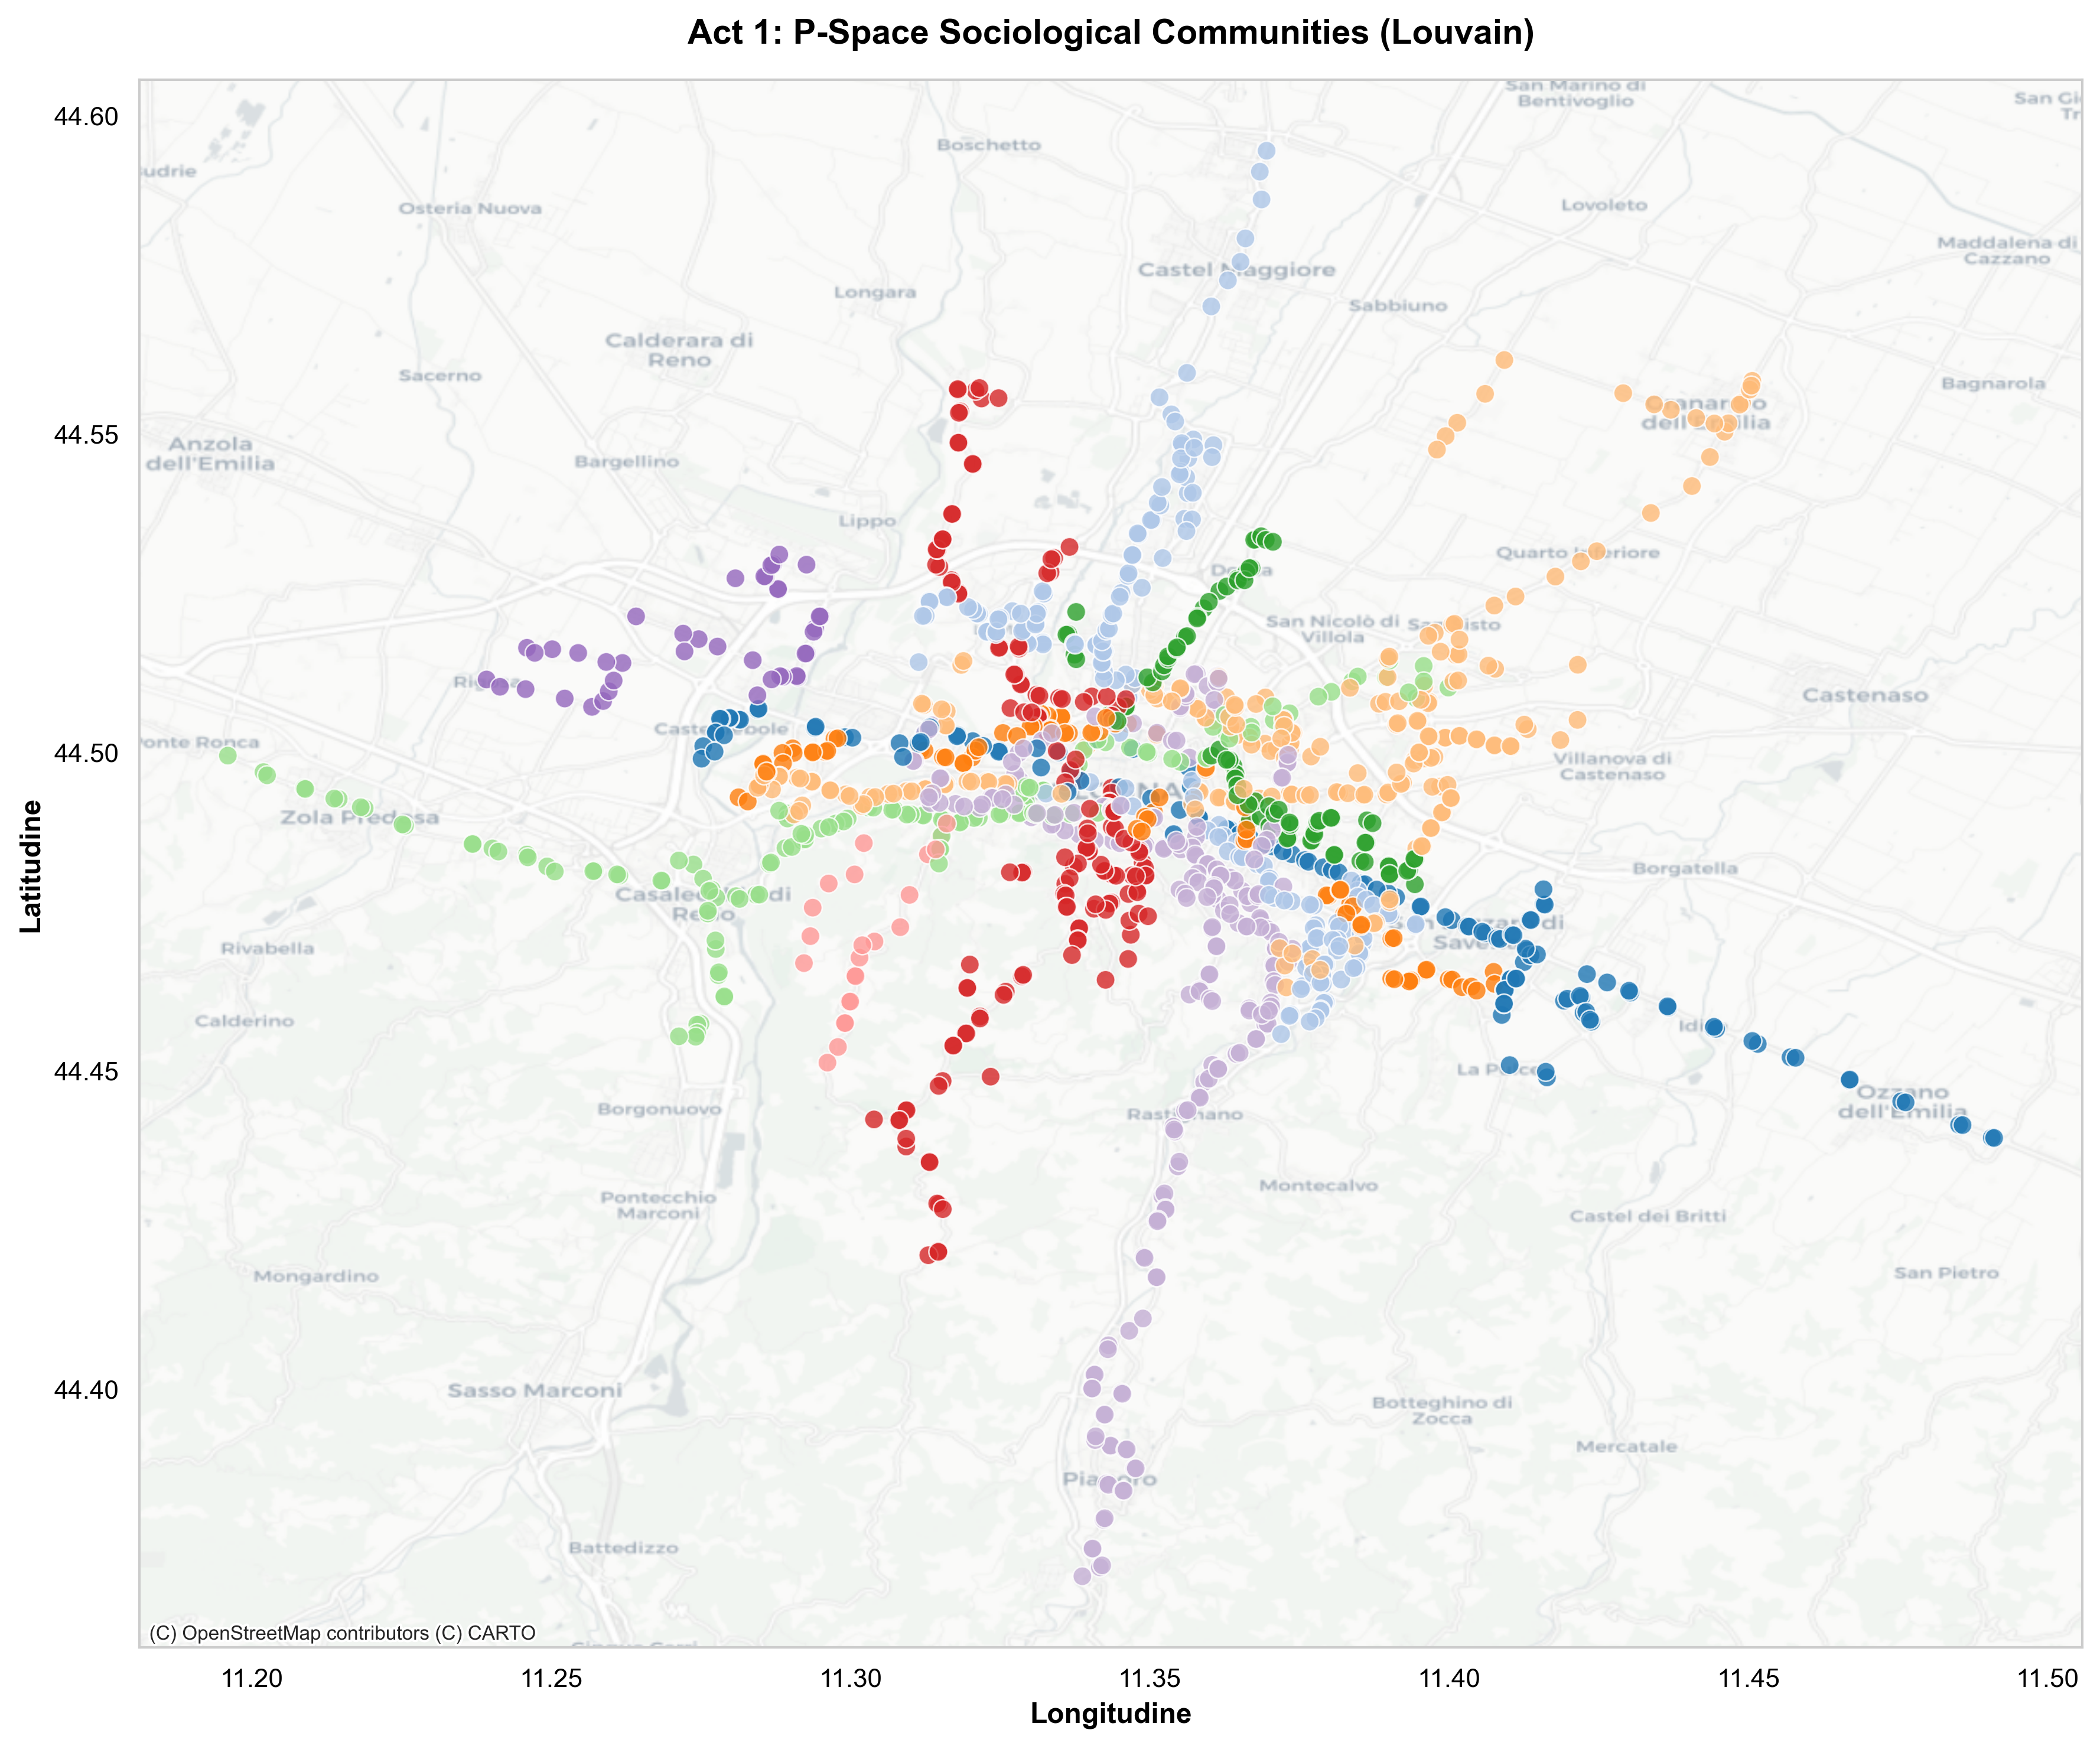
\includegraphics[width=\textwidth]{figures/bologna/bologna_communities_map.png}
        \caption{Community detection (Louvain) on the Bus Only P-space.}
        \label{fig:communities}
    \end{minipage}
    \hfil
    \begin{minipage}{0.48\textwidth}
        \centering
        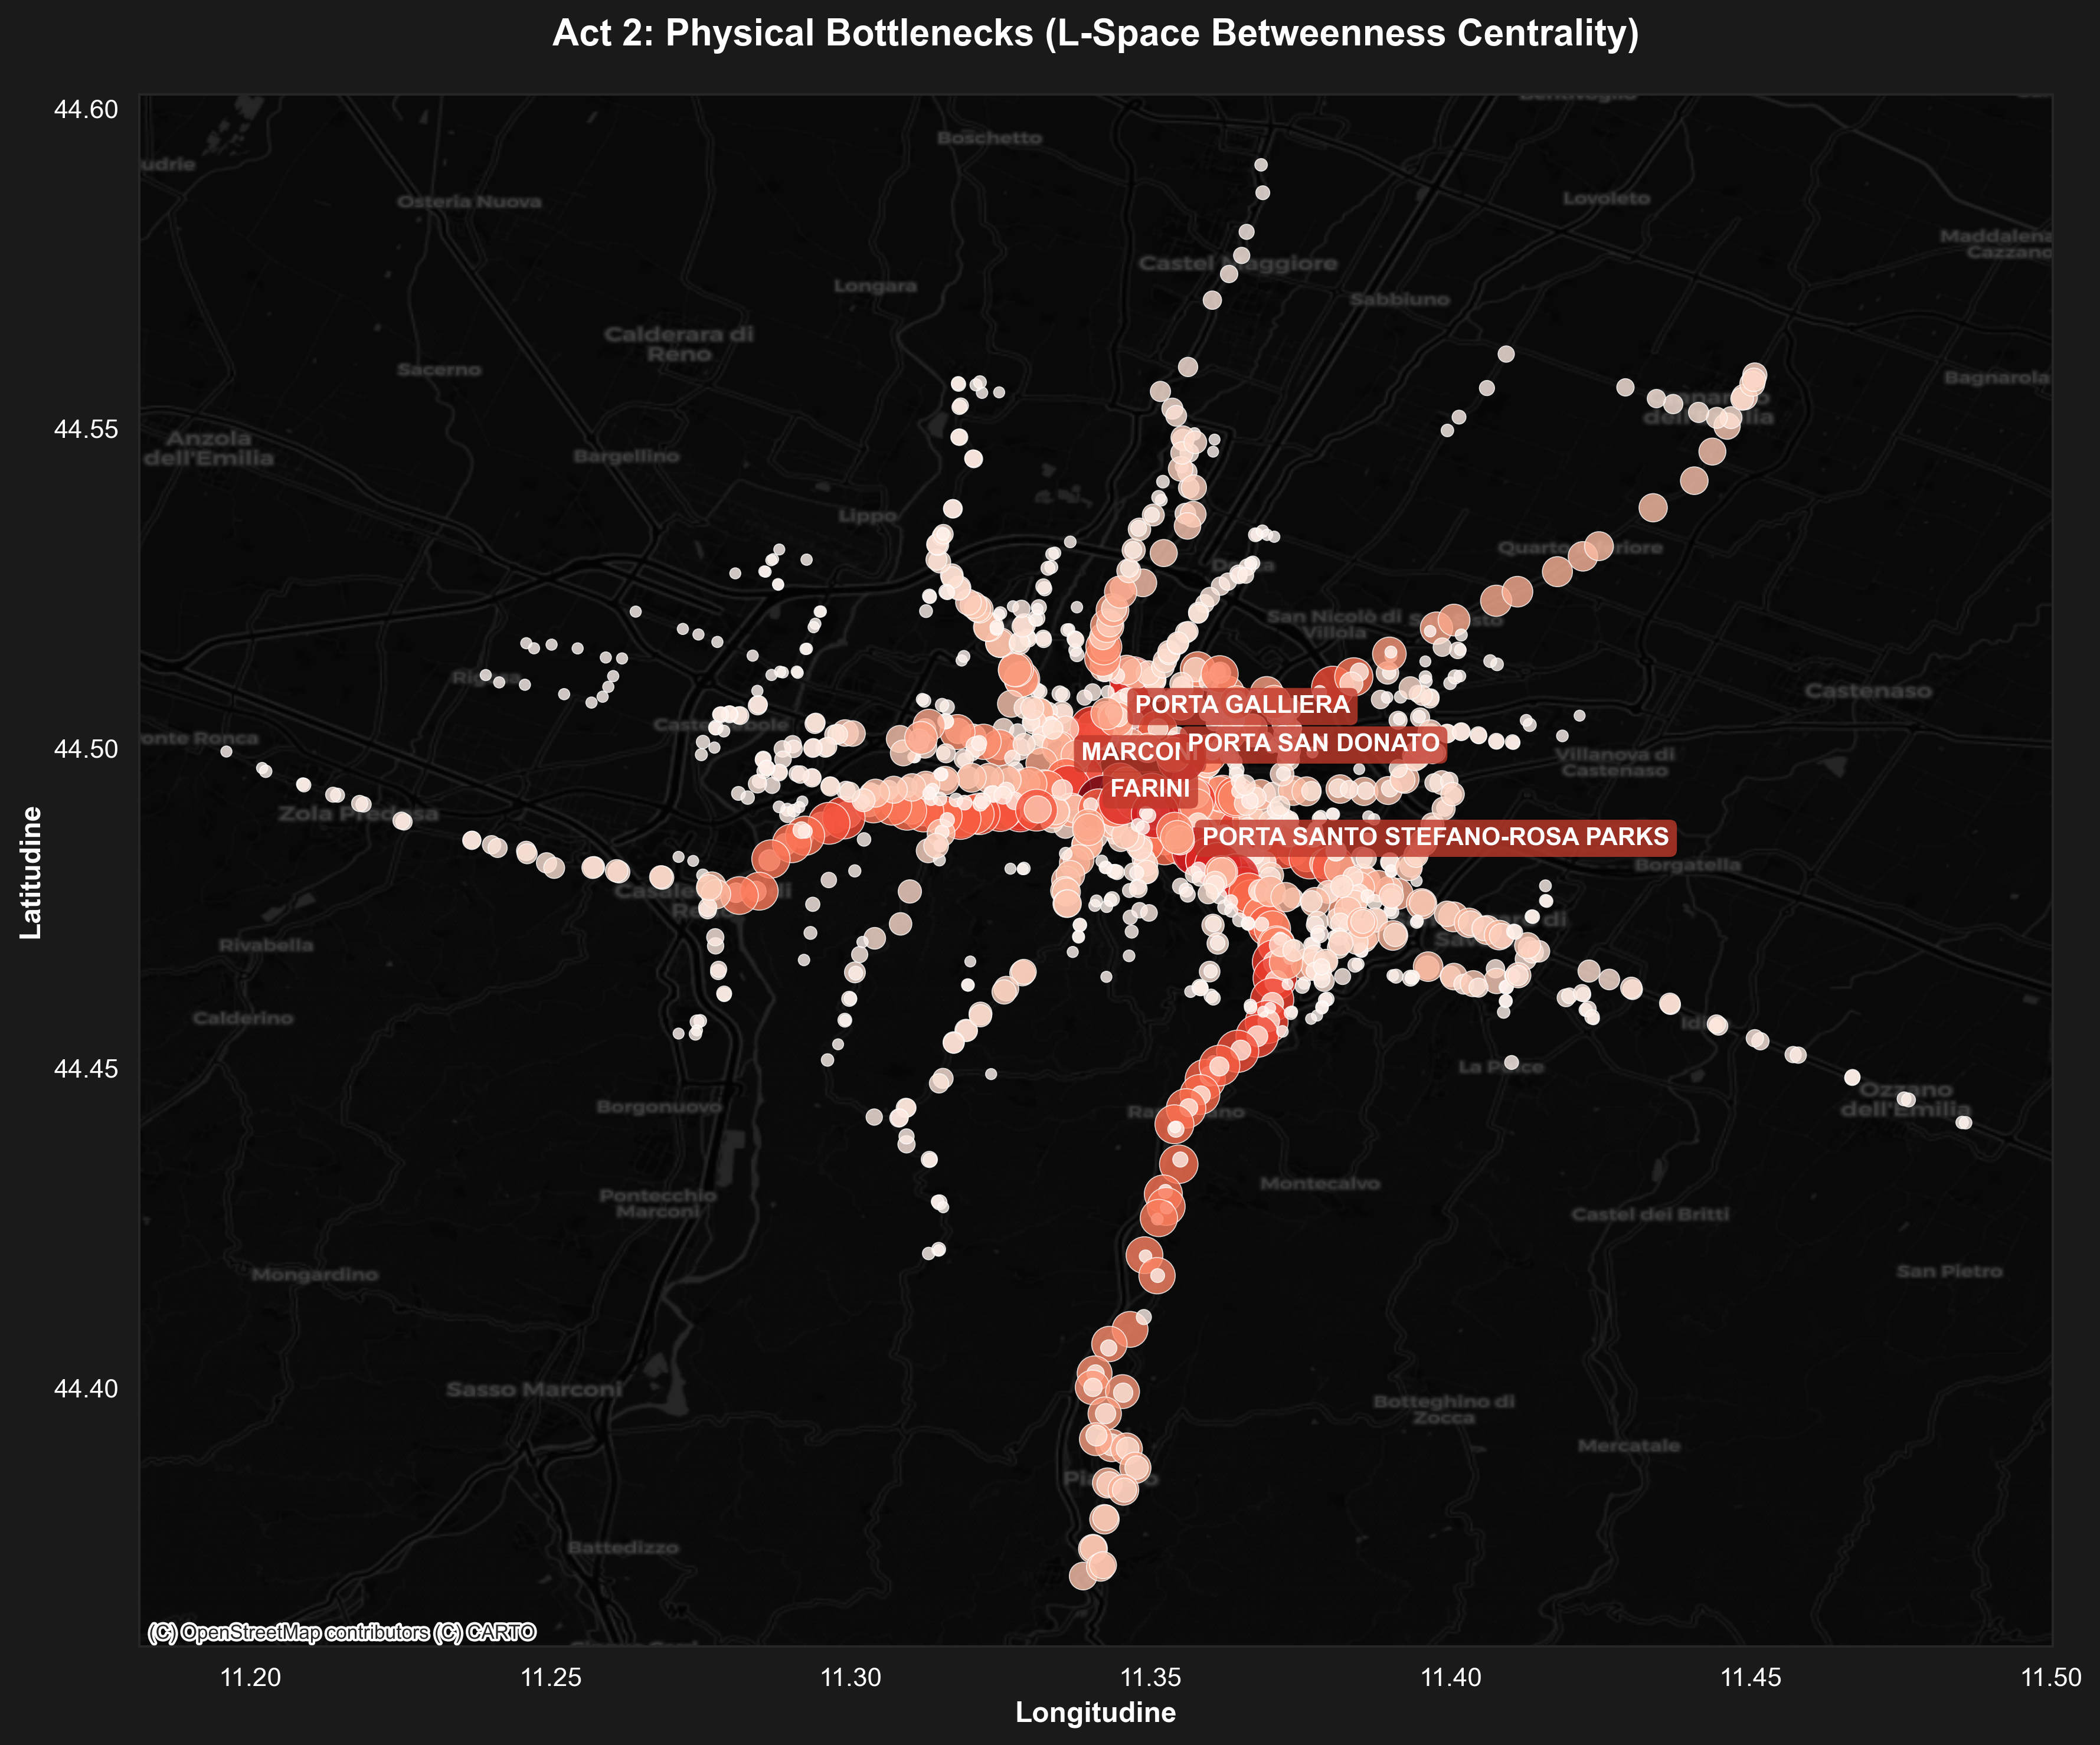
\includegraphics[width=\textwidth]{figures/bologna/bologna_bottlenecks_map.png}
        \caption{Spatial distribution of L-space betweenness centrality.}
        \label{fig:bottlenecks_map}
    \end{minipage}
\end{figure}

To further investigate the topological character of these bottlenecks, we analyze the relationship between node degree and betweenness centrality. Figure~\ref{fig:centrality_scatter} shows a regression plot of betweenness centrality against node degree. Since degree is a discrete quantity in L-space (most stations have degree 2 or 4, corresponding to the transit lines passing through them), a horizontal jitter of $0.15$ was applied to reveal the true density distribution of the points.

The regression lines capture the general positive trend. Crucially, the top-5 physical bottlenecks are prominent outliers lying far above the trend. This demonstrates that in spatial networks a node's local connectivity (degree) is an insufficient proxy for its global routing importance (betweenness), which is instead governed by geographic barriers, historical city gates, and bridge corridors.

\begin{figure}[H]
    \centering
    \begin{minipage}{0.48\textwidth}
        \centering
        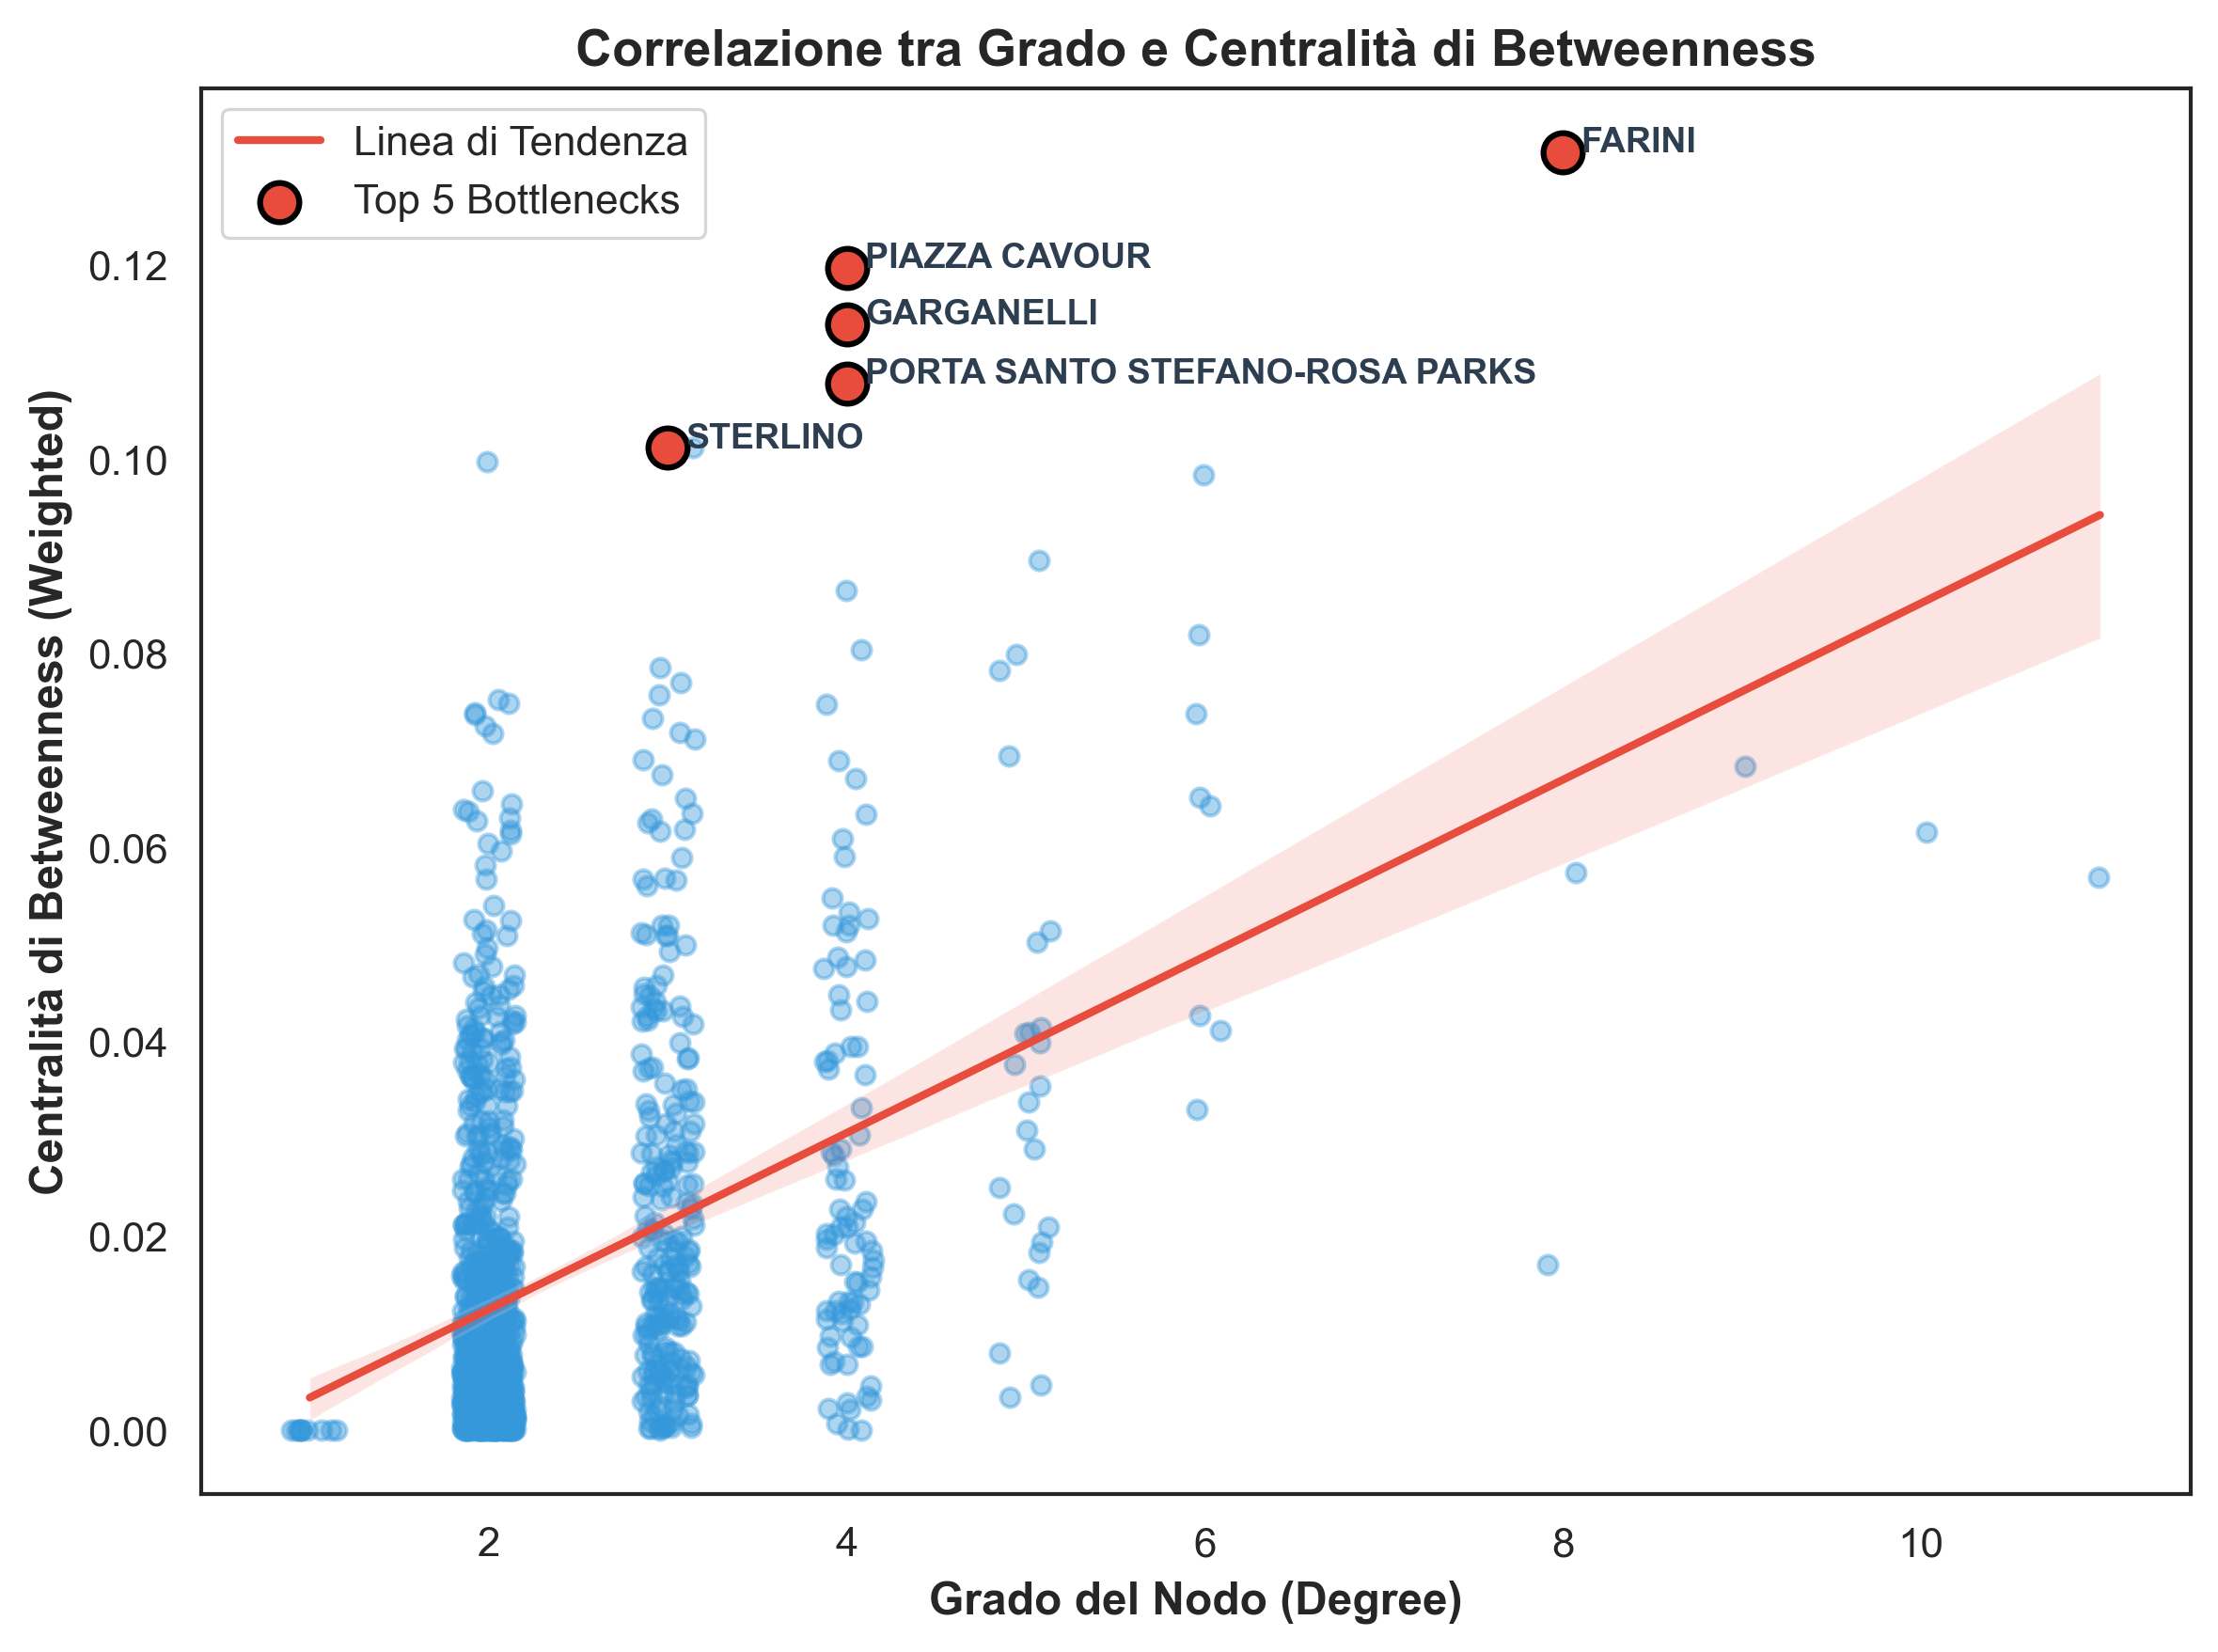
\includegraphics[width=\textwidth]{figures/bologna/bologna_centrality_scatter.png}
        \caption{Degree vs betweenness centrality. Jitter is applied to show density; top-5 bottlenecks are highlighted.}
        \label{fig:centrality_scatter}
    \end{minipage}
    \hfill
    \begin{minipage}{0.48\textwidth}
        \centering
        
\includegraphics[width=\textwidth]{figures/bologna/bologna_betweenness_hist.png}
        \caption{Betweenness distribution (values $>0$) with a KDE curve, indicating a heavy-tailed bottleneck topology.}
        \label{fig:betweenness_hist}
    \end{minipage}
\end{figure}

Figure~\ref{fig:betweenness_hist} presents the probability density of betweenness centrality values greater than zero. The distribution is highly right-skewed and heavy-tailed: the vast majority of nodes have negligible betweenness, whereas a tiny elite of bottlenecks controls the transit flows across the municipal area.

\subsubsection{Macroscopic Analysis: Small-Worldness and Efficiency}
We computed the average shortest-path travel time ($L$), the clustering coefficient ($C$, calculated on the giant component for mathematical consistency), the global efficiency ($E_{glob}$)~\cite{latora}, the small-world index $\sigma$ (Watts--Strogatz-type comparison against Erd\H{o}s--R\'enyi null models of matched size and density), and Telesford's small-world index $\omega$~\cite{telesford} for the two baseline scenarios (Table~\ref{tab:macroscopic}). All metrics are computed on demographically loaded travel times, i.e.\ with the dynamic dwell-time penalties of Section~\ref{validity-and-reliability} applied uniformly; the topological indices $\sigma$ and $\omega$ are computed on the unweighted topology (hop distances) of the giant component.

\begin{table}[H]
    \centering
    \caption{Macroscopic Network Metrics and Null-Model Comparison (under demographic load)}
    \label{tab:macroscopic}
    \begin{tabular}{lcc}
        \toprule
        Metric & Bus Only & Planned Tram \\
        \midrule
        Nodes ($N_{lcc}$) & 1212 & 1283 \\
        Edges ($M_{lcc}$) & 1482 & 1570 \\
        Avg Travel Time $L$ (sec) & 2162.69 & 2183.89 \\
        Clustering Coeff ($C$) & 0.0113 & 0.0124 \\
        Global Efficiency $E_{glob}$ ($\text{s}^{-1}$) & 0.000658 & 0.000690 \\
        Small-World Sigma ($\sigma$) & 2.35 & 4.29 \\
        Small-World Omega ($\omega$) & 0.00 & 0.00 \\
        \bottomrule
    \end{tabular}
\end{table}

The baseline bus network has a giant component of 1212 nodes. The Planned Tram scenario expands the component to 1283 nodes by adding 71 new peripheral or previously disconnected stops.
In terms of cohesion, the L-space giant component is extremely sparse (density $\approx 0.002$), as expected of street-constrained, quasi-planar infrastructure, whereas the P-space is two orders of magnitude denser (density $\approx 0.10$). Regarding scale freedom, the L-space degree distribution is inherently narrow ($\langle k \rangle \approx 2.4$), so no strict power law can emerge; in P-space, the degree distribution is broad and right-skewed (median 115, maximum 663 at the central corridor hubs), consistent with the hub-dominated, ``scale-free-like'' organization reported for metro systems~\cite{derrible}, although the clique-based construction bounds the minimum degree and precludes a formal power-law fit.
The small-world index $\sigma$ is greater than 1 in both scenarios, indicating small-world properties. The collapse of Telesford's omega ($\omega = 0.00$)~\cite{telesford} is a structural property of L-space transit networks: because transit lines are linear chains, the average node degree is $\langle k \rangle \approx 2.4$. The reference regular lattice generated to match this degree has $k = 2$ (a simple cycle), whose clustering coefficient is $C_{lat} = 0$, making the ratio $C/C_{lat}$ in Telesford's formula undefined (the pipeline reports $\omega = 0$ in this case). The index $\sigma$ therefore remains the more informative indicator of small-worldness here.

\subsubsection{Resilience Stress-Tests}
We first simulated a \textbf{dynamic targeted attack} in which centralities are recalculated at each removal step. Table~\ref{tab:targeted_attack} details the sequential efficiency drops and the specific bottleneck removed at each step for the two baseline networks. (PORTA SAN DONATO appears twice for the Bus Only network because two distinct physical stops share that name.)

\begin{table}[H]
    \centering
    \caption{Global Efficiency Drop (\%) under Dynamic Targeted Bottleneck Attack}
    \label{tab:targeted_attack}
    \begin{tabular}{cll}
        \toprule
        Step & Bus Only & Planned Tram \\
        \midrule
        1 & -0.63\% (FARINI) & -0.59\% (FARINI) \\
        2 & -1.54\% (MARCONI) & -2.37\% (PIAZZA DELL'UNITA') \\
        3 & -2.79\% (PIAZZA MALPIGHI) & -3.21\% (MARCONI) \\
        4 & -3.29\% (PORTA SAN DONATO) & -4.45\% (PIAZZA MALPIGHI) \\
        5 & -4.03\% (PORTA SAN DONATO) & -4.93\% (PORTA SAN DONATO) \\
        \bottomrule
    \end{tabular}
\end{table}

We then performed a global percolation simulation on the baseline network comparing three ``operative stress'' scenarios: random failure, accidents (removal probabilities weighted by historical accident counts), and targeted attack (removing nodes in decreasing order of initial betweenness centrality). Figure~\ref{fig:resilience} shows the percolation curves.

\begin{figure}[H]
    \centering
    
\includegraphics[width=0.95\textwidth]{figures/bologna/bologna_resilience_curves.png}
    \caption{Operative stress: percolation curves on the bus network. Left: topological fragmentation. Right: dynamic efficiency loss.}
    \label{fig:resilience}
\end{figure}

The percolation curves reveal a classic spatial-network phenomenon. Under targeted attack, global efficiency collapses much faster than the physical size of the largest connected component (LCC). After removing $5\%$ of the top-betweenness nodes, the LCC still spans $88.83\%$ of the network's nodes, so the network remains largely connected; global efficiency, however, has already crashed by $27.43\%$ (down to $72.57\%$ of the baseline). Removing the core bottlenecks (such as Farini, Marconi, and Piazza Malpighi) forces passengers onto long, circuitous detours, degrading overall transit utility well before the network physically fragments. By the time $10\%$ of the targeted hubs are removed, global efficiency has dropped by $41.84\%$ (residual efficiency $58.16\%$).

In contrast, the network is highly resilient to random failures and accident-driven blockages. At $5\%$ removal, random failures cause a modest $14.19\%$ drop in global efficiency, and accident-weighted removals a similar $14.92\%$ drop. Accidents and random failures mostly hit the large population of low-betweenness peripheral nodes, which are topologically redundant and have minimal impact on global routing.

To evaluate the ``exogenous stress'' dimension, we overlaid the demographic population data directly onto the network topology, adjusting station dwell times dynamically according to passenger pressure (Figure~\ref{fig:demographic_pressure}).

\begin{figure}[H]
    \centering
    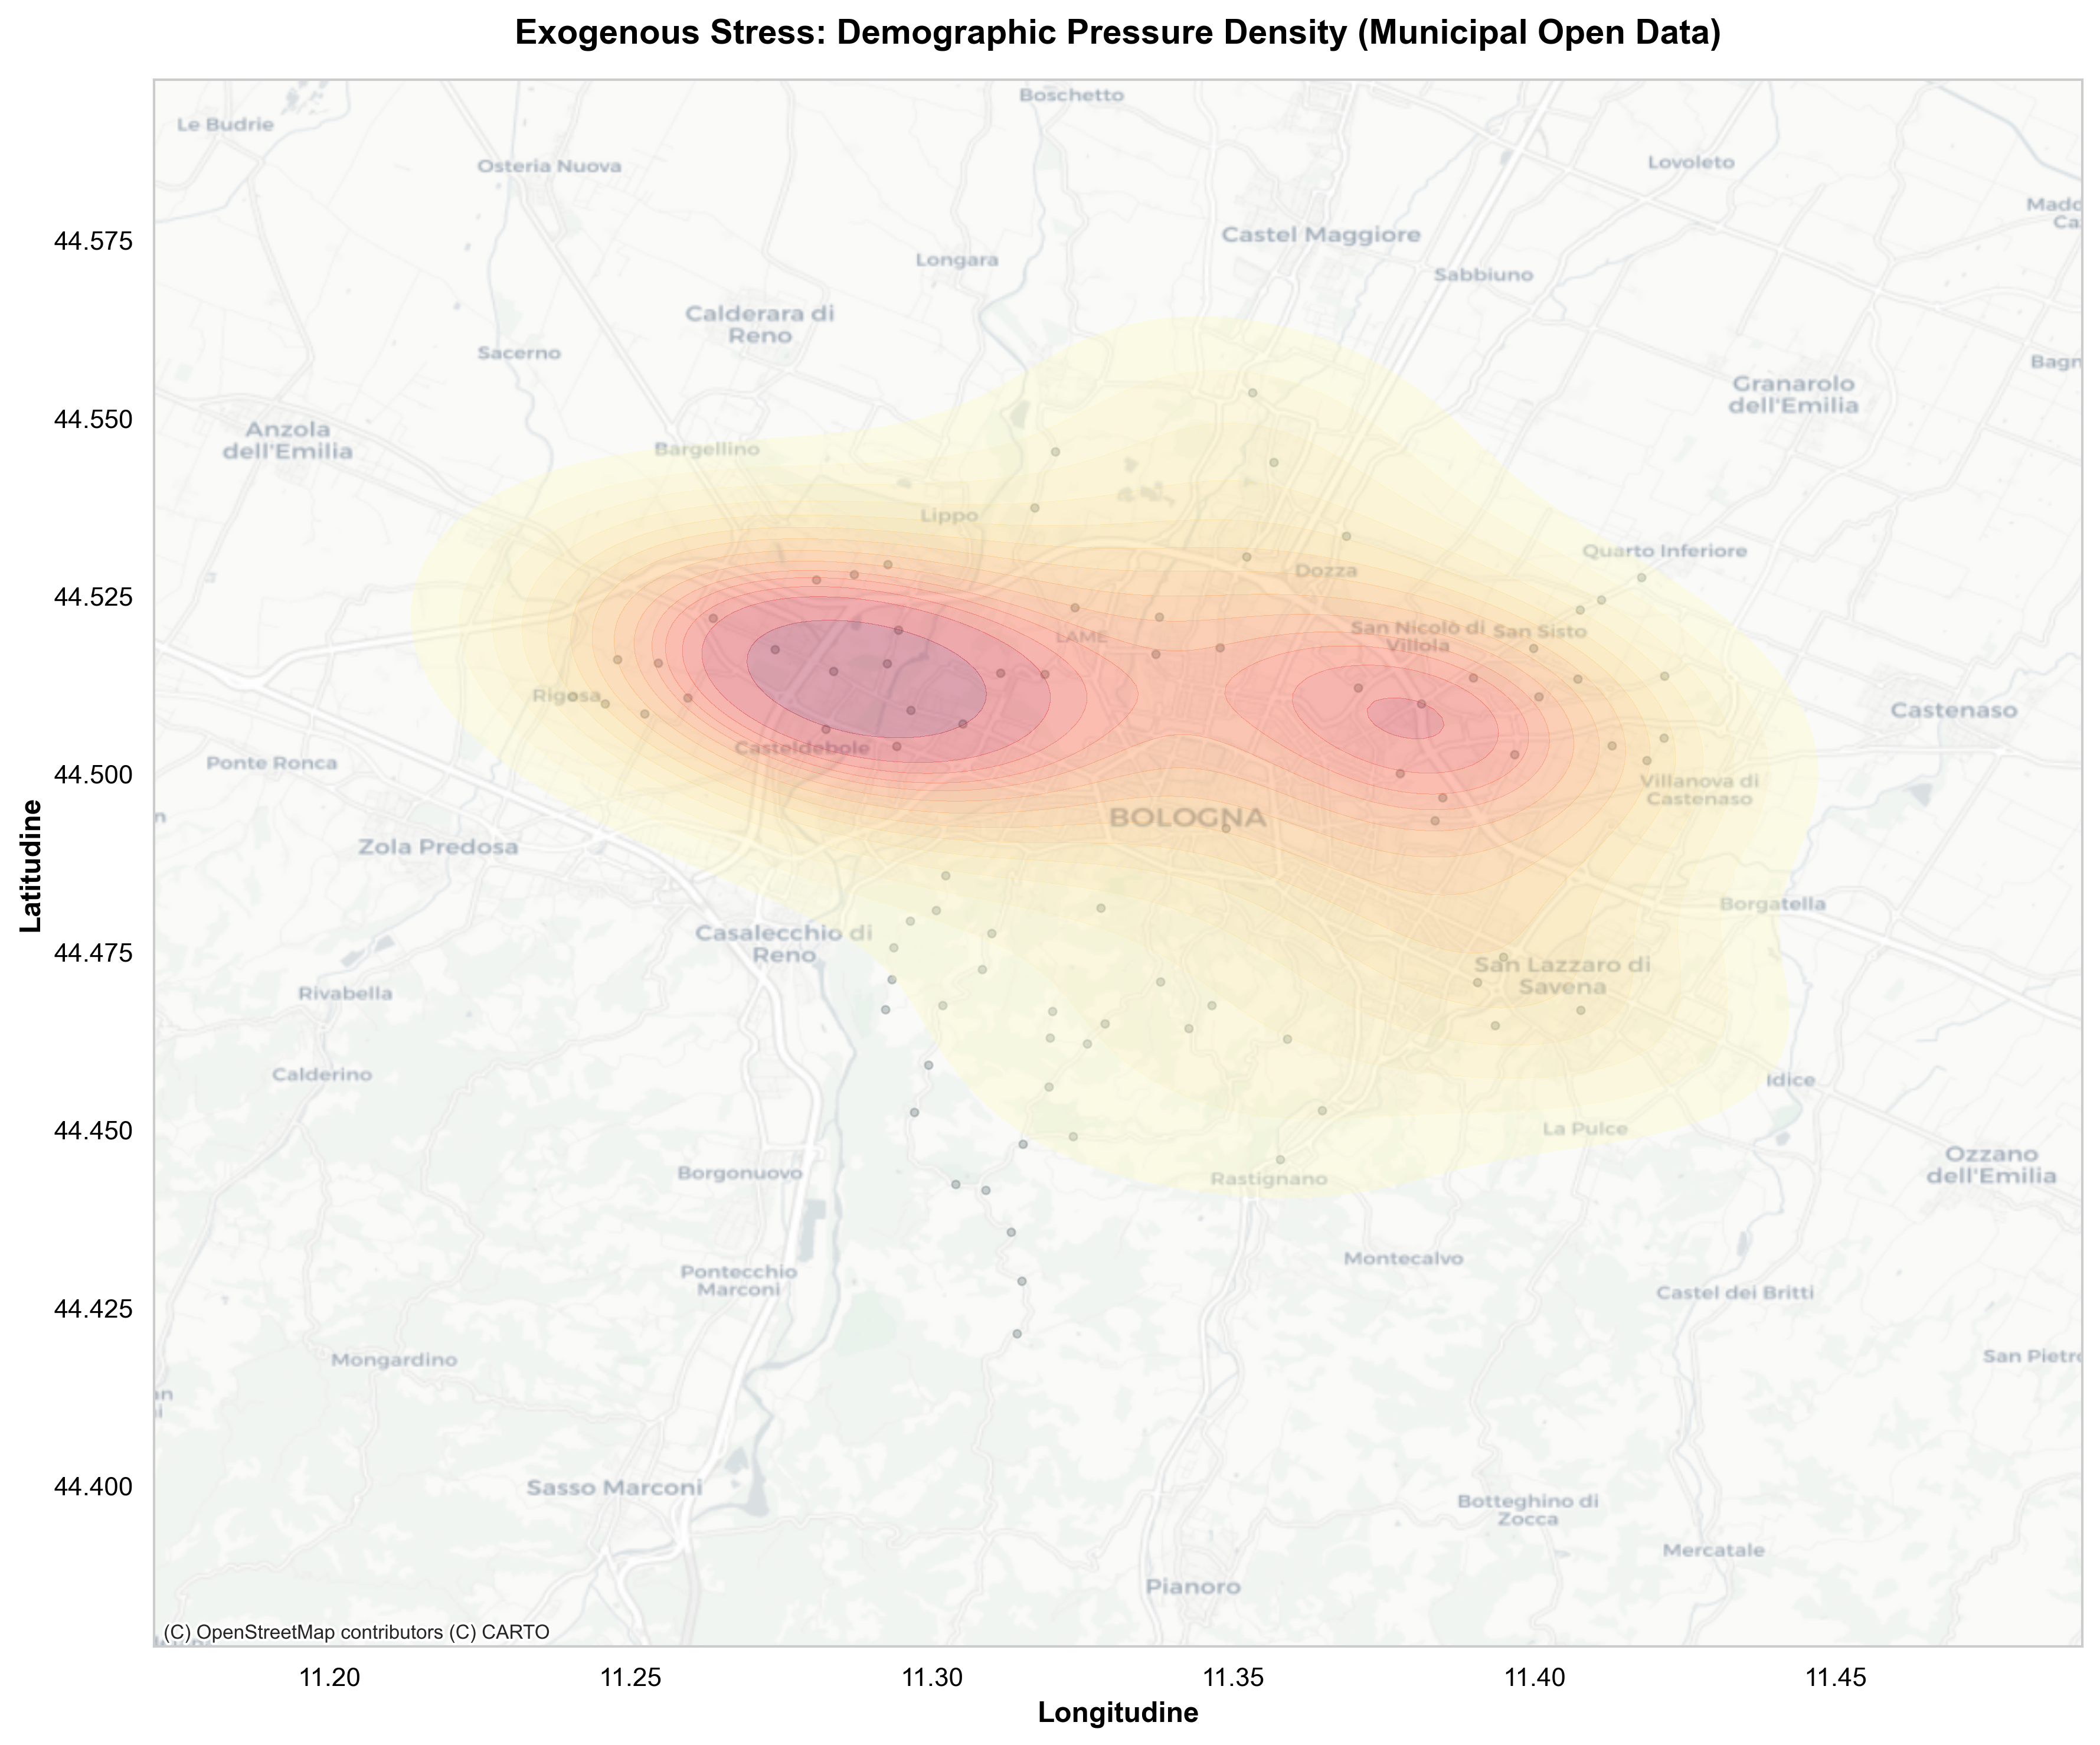
\includegraphics[width=0.85\textwidth]{figures/bologna/bologna_demographic_pressure_map.png}
    \caption{Exogenous stress: demographic pressure density overlaid on the network, highlighting suburban areas (e.g., Borgo Panigale) with heavy residential loads.}
    \label{fig:demographic_pressure}
\end{figure}

\subsubsection{Interim Baseline Conclusions}
The baseline study reveals a subtle insight: while the Planned Tram scenario increases global efficiency $E_{glob}$ from $0.000658$ to $0.000690\text{ s}^{-1}$ (thanks to fast central links), it slightly increases the average travel time $L$ from $2162.69$ to $2183.89\text{ s}$. This is a structural effect of expanding the giant component (71 additional peripheral stops), which adds long peripheral paths and inflates the arithmetic mean. Under targeted attack, the planned tramway yields a modest resilience benefit in the intermediate removal range, but it does not resolve the core centrality chokepoints of the historic centre (Figure~\ref{fig:comparative_resilience}).

\begin{figure}[H]
    \centering
    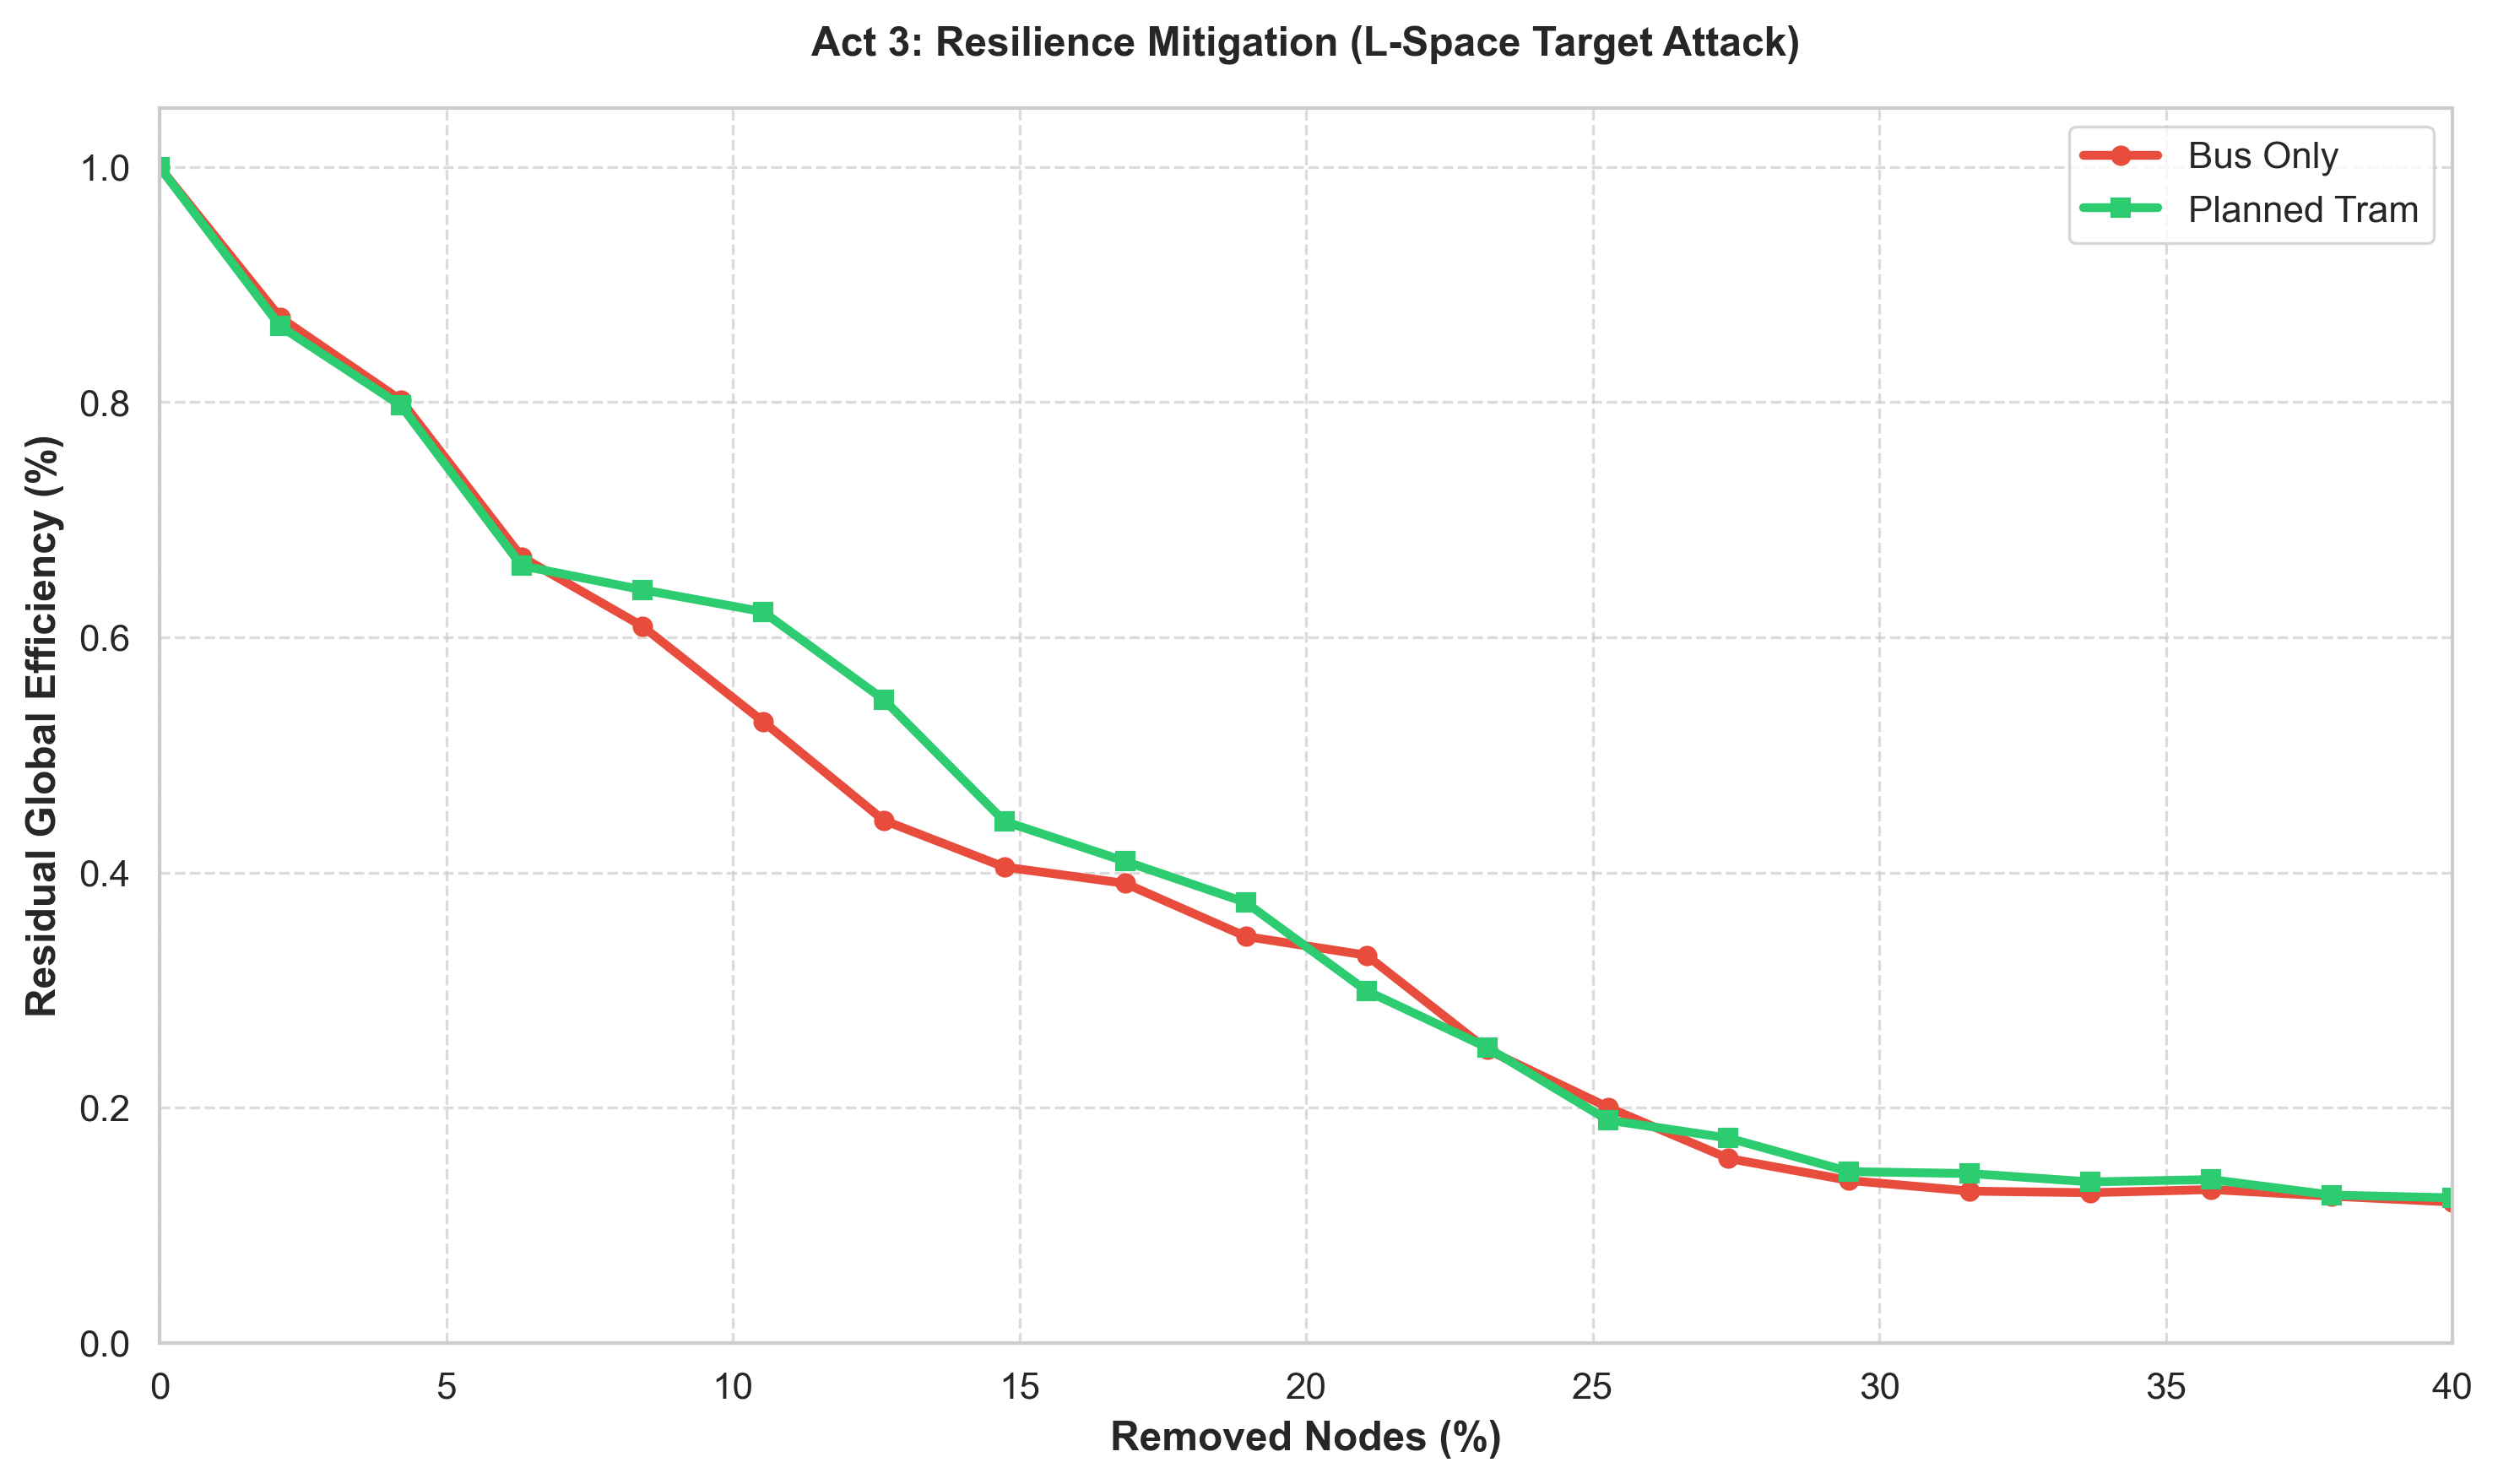
\includegraphics[width=0.85\textwidth]{figures/bologna/bologna_resilience_comparison.png}
    \caption{Comparative resilience under targeted attack. The Planned Tram network (green) retains slightly higher residual efficiency than Bus Only (red) in the intermediate removal range ($\approx$8--15\% of nodes); the curves largely overlap elsewhere.}
    \label{fig:comparative_resilience}
\end{figure}

\subsection{Future Scenarios Exploration}
\label{scenarios-exploration}
To explore alternative transit strategies and optimize the planned network, we evaluate two additional future scenarios.

\subsubsection{Scenario A: Circular Ring-Road Tramway (Lines 32 and 33)}
This scenario upgrades the circular ring-road bus corridor (Line 32 clockwise and Line 33 counter-clockwise) into a fast, dedicated tramway running along the \textit{viali di circonvallazione}, in addition to the Planned Tram radial layout. The Circular Tram connects the major suburban radial lines while bypassing the historic core entirely.

\subsubsection{Scenario B: Algorithmic Optimal Tramway (TNDP)}
To support spatial planning from an algorithmic perspective, we implemented a greenfield optimization model that designs a new tramway network from scratch under a total length budget of $25\text{ km}$. This falls under the classical Transit Network Design Problem (TNDP), which is non-convex and NP-hard~\cite{fan, jha}. The algorithm selects two central seed hubs --- \textit{Farini} and \textit{Piazza Cavour}, the two highest-scoring nodes by combined betweenness and demographic weight --- and greedily grows tram segments from the active network by repeatedly converting the adjacent bus edge with the best utility-per-metre ratio, where the multi-criteria edge utility is
$$U(e) = \alpha \cdot EB(e) + \beta \cdot \Delta t(e) \cdot EB(e) + \gamma \cdot \text{avg\_pop}(e)$$
with $\alpha=\beta=\gamma=1$, assuming an equal baseline weighting for topological importance, travel-time savings, and demographic coverage. Here $EB(e)$ is the edge betweenness, $\Delta t(e)$ the travel-time saving from tram conversion, and $\text{avg\_pop}(e)$ the average population served by the edge's endpoints; each component is normalized to $[0, 1]$ by Min--Max scaling across all edges to guarantee dimensional consistency. The resulting layout, a single 24.85 km corridor network through the densest and most central axes, is shown in Figure~\ref{fig:optimized_layout}.

\begin{figure}[H]
    \centering
    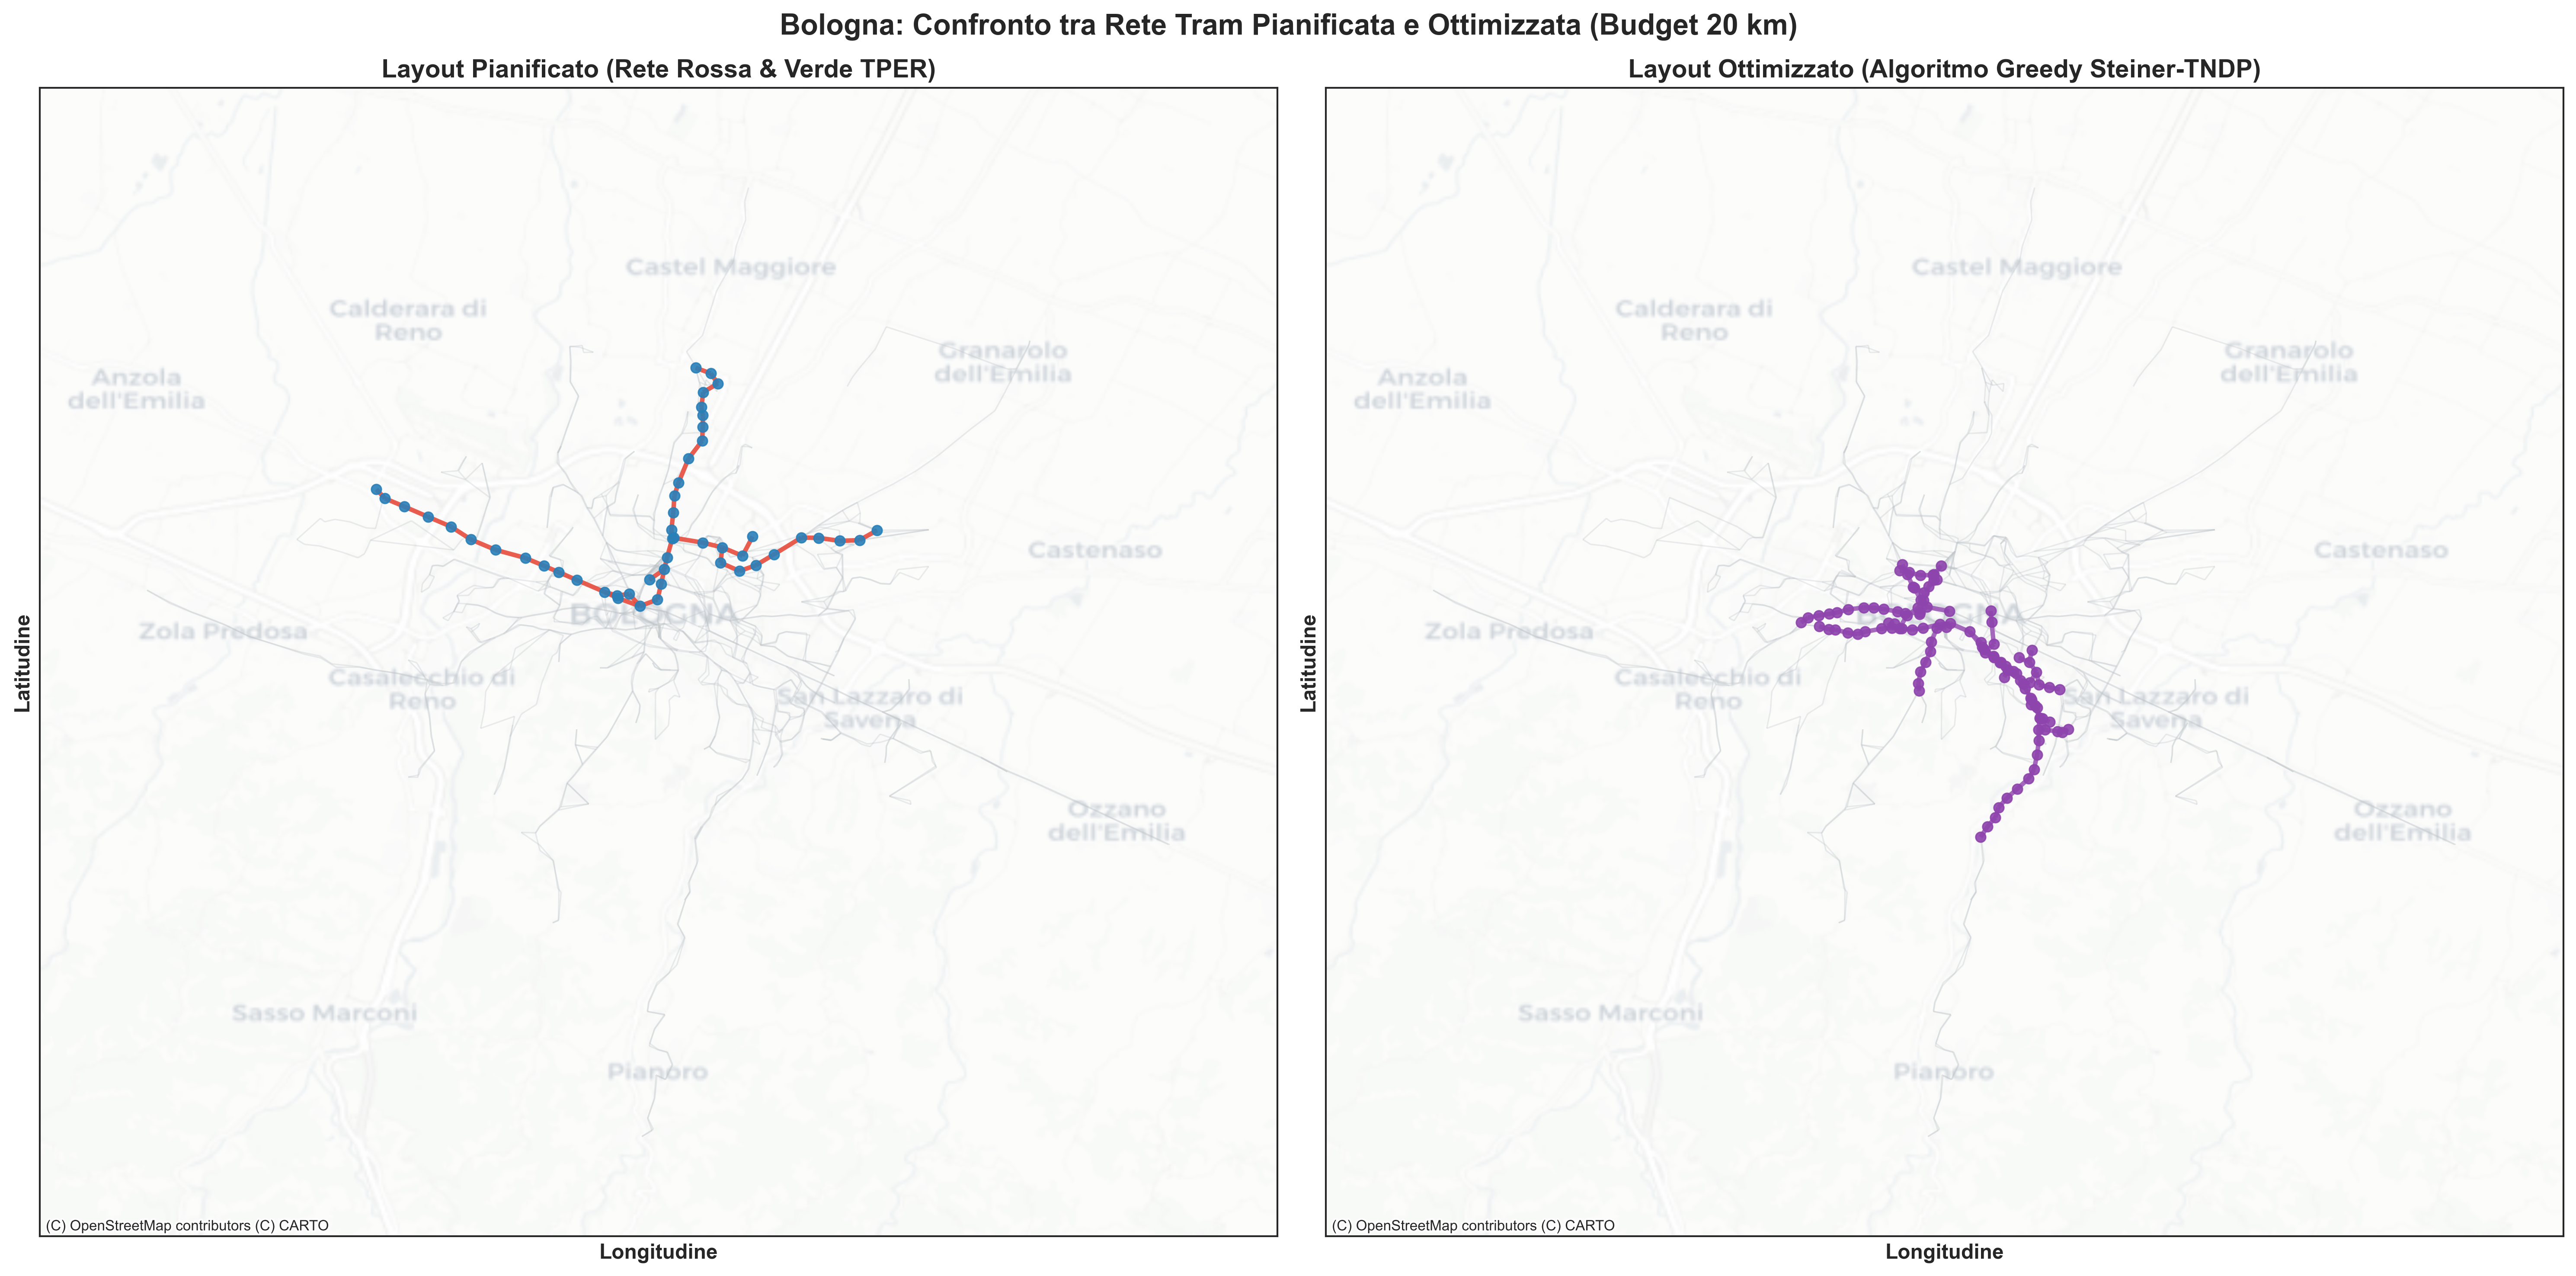
\includegraphics[width=0.85\textwidth]{figures/bologna/bologna_optimized_layout.png}
    \caption{Optimal tramway layout designed by the greedy TNDP algorithm under a 25 km budget, routed along high-density and high-betweenness corridors.}
    \label{fig:optimized_layout}
\end{figure}

\subsubsection{Comparative Performance under Demographic Load}
Table~\ref{tab:tram_optimization} compares the performance of the four scenarios. All metrics are computed under the same demographic load as Table~\ref{tab:macroscopic} (dynamic dwell times applied uniformly), so the four rows are directly comparable.

\begin{table}[H]
    \centering
    \caption{Comparative Performance of Network Scenarios under Demographic Load}
    \label{tab:tram_optimization}
    \setlength{\tabcolsep}{5pt}
    \begin{tabular}{lccc}
        \toprule
        Scenario & \shortstack{Avg Travel Time\\$L$ (sec)} & \shortstack{Global Efficiency\\$E_{glob}$ ($\text{s}^{-1}$)} & \shortstack{Tram Population\\served} \\
        \midrule
        Bus Only & 2162.69 & 0.000658 & N/A \\
        Planned Tram & 2183.89 & 0.000690 & 33,106 \\
        Circular Tram & 2155.92 & 0.000702 & 45,227 \\
        Optimal Tram & 2060.40 & 0.000688 & 42,230 \\
        \bottomrule
    \end{tabular}
\end{table}

The Circular Tram achieves the highest global efficiency ($0.000702\text{ s}^{-1}$) by adding a fast orbital bypass that shortens a large number of inter-sector trips. The Optimal Tram, in turn, achieves the lowest average travel time ($2060.40\text{ s}$, about $4.7\%$ faster than the Bus Only baseline over the same stop set) while directly serving \textbf{42,230 residents} at its stations --- a \textbf{27.6\% increase} in coverage over the Planned Tram layout ($33,106$ residents). Because the greedy algorithm upgrades existing high-betweenness bus corridors rather than adding new peripheral stops, it accelerates the network without enlarging the giant component.

This performance gap highlights a crucial planning insight: the Planned Tram extends into peripheral radial corridors, maximizing municipal reach but adding long routes that inflate average travel times. In contrast, the optimization concentrates the $25\text{ km}$ budget precisely along the high-betweenness, high-congestion, and high-density corridors of the inner urban ring and main radial paths. Topology-driven design models can therefore improve both commuter travel times and population coverage per unit of infrastructure built.

\subsubsection{Commuter Shock: Forced Passenger Hub Injection}
To evaluate how these infrastructures absorb massive commuter congestion, we mapped the Planned Tram layout (Figure~\ref{fig:tram_impact_map}) and ran a forced passenger injection simulation at \textit{Stazione Centrale} and the \textit{Autostazione}, Bologna's main inter-modal hubs.

\begin{figure}[H]
    \centering
    \begin{minipage}{0.48\textwidth}
        \centering
        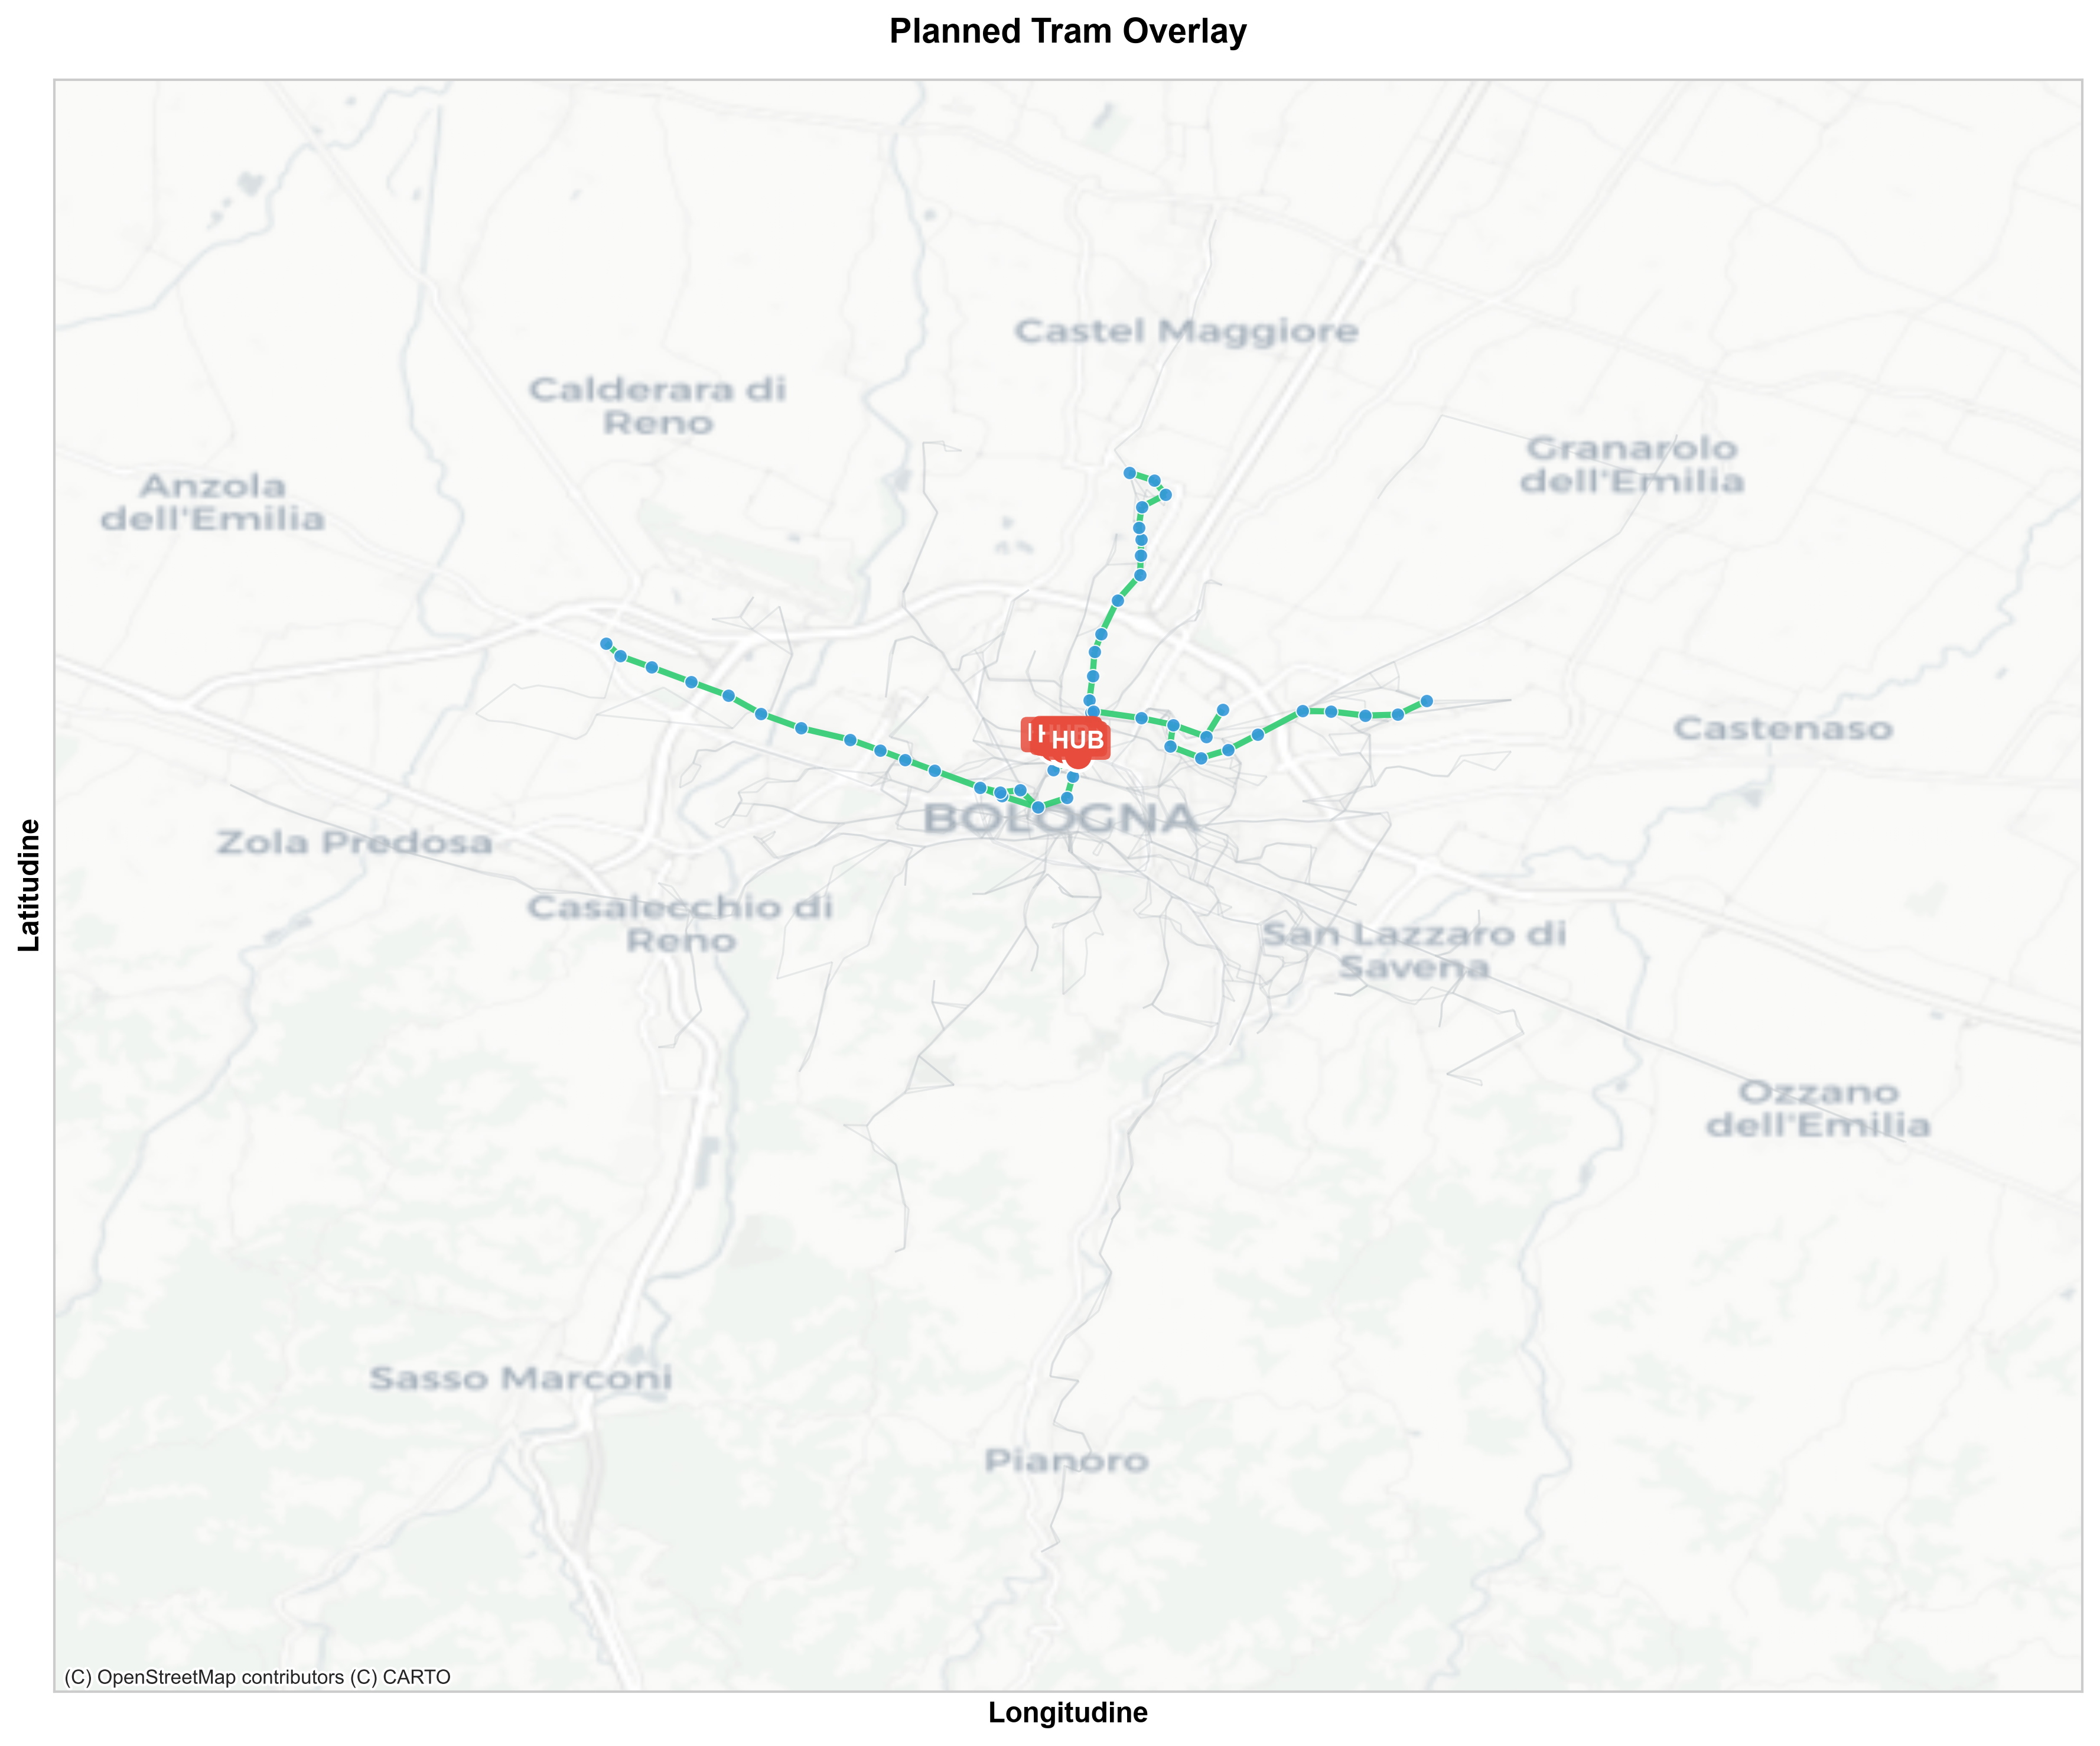
\includegraphics[width=\textwidth]{figures/bologna/bologna_tram_impact_map.png}
        \caption{Isolated layout of the Planned Tram lines (Red and Green), highlighting the Stazione Centrale and Autostazione hubs.}
        \label{fig:tram_impact_map}
    \end{minipage}
    \hfill
    \begin{minipage}{0.48\textwidth}
        \centering
        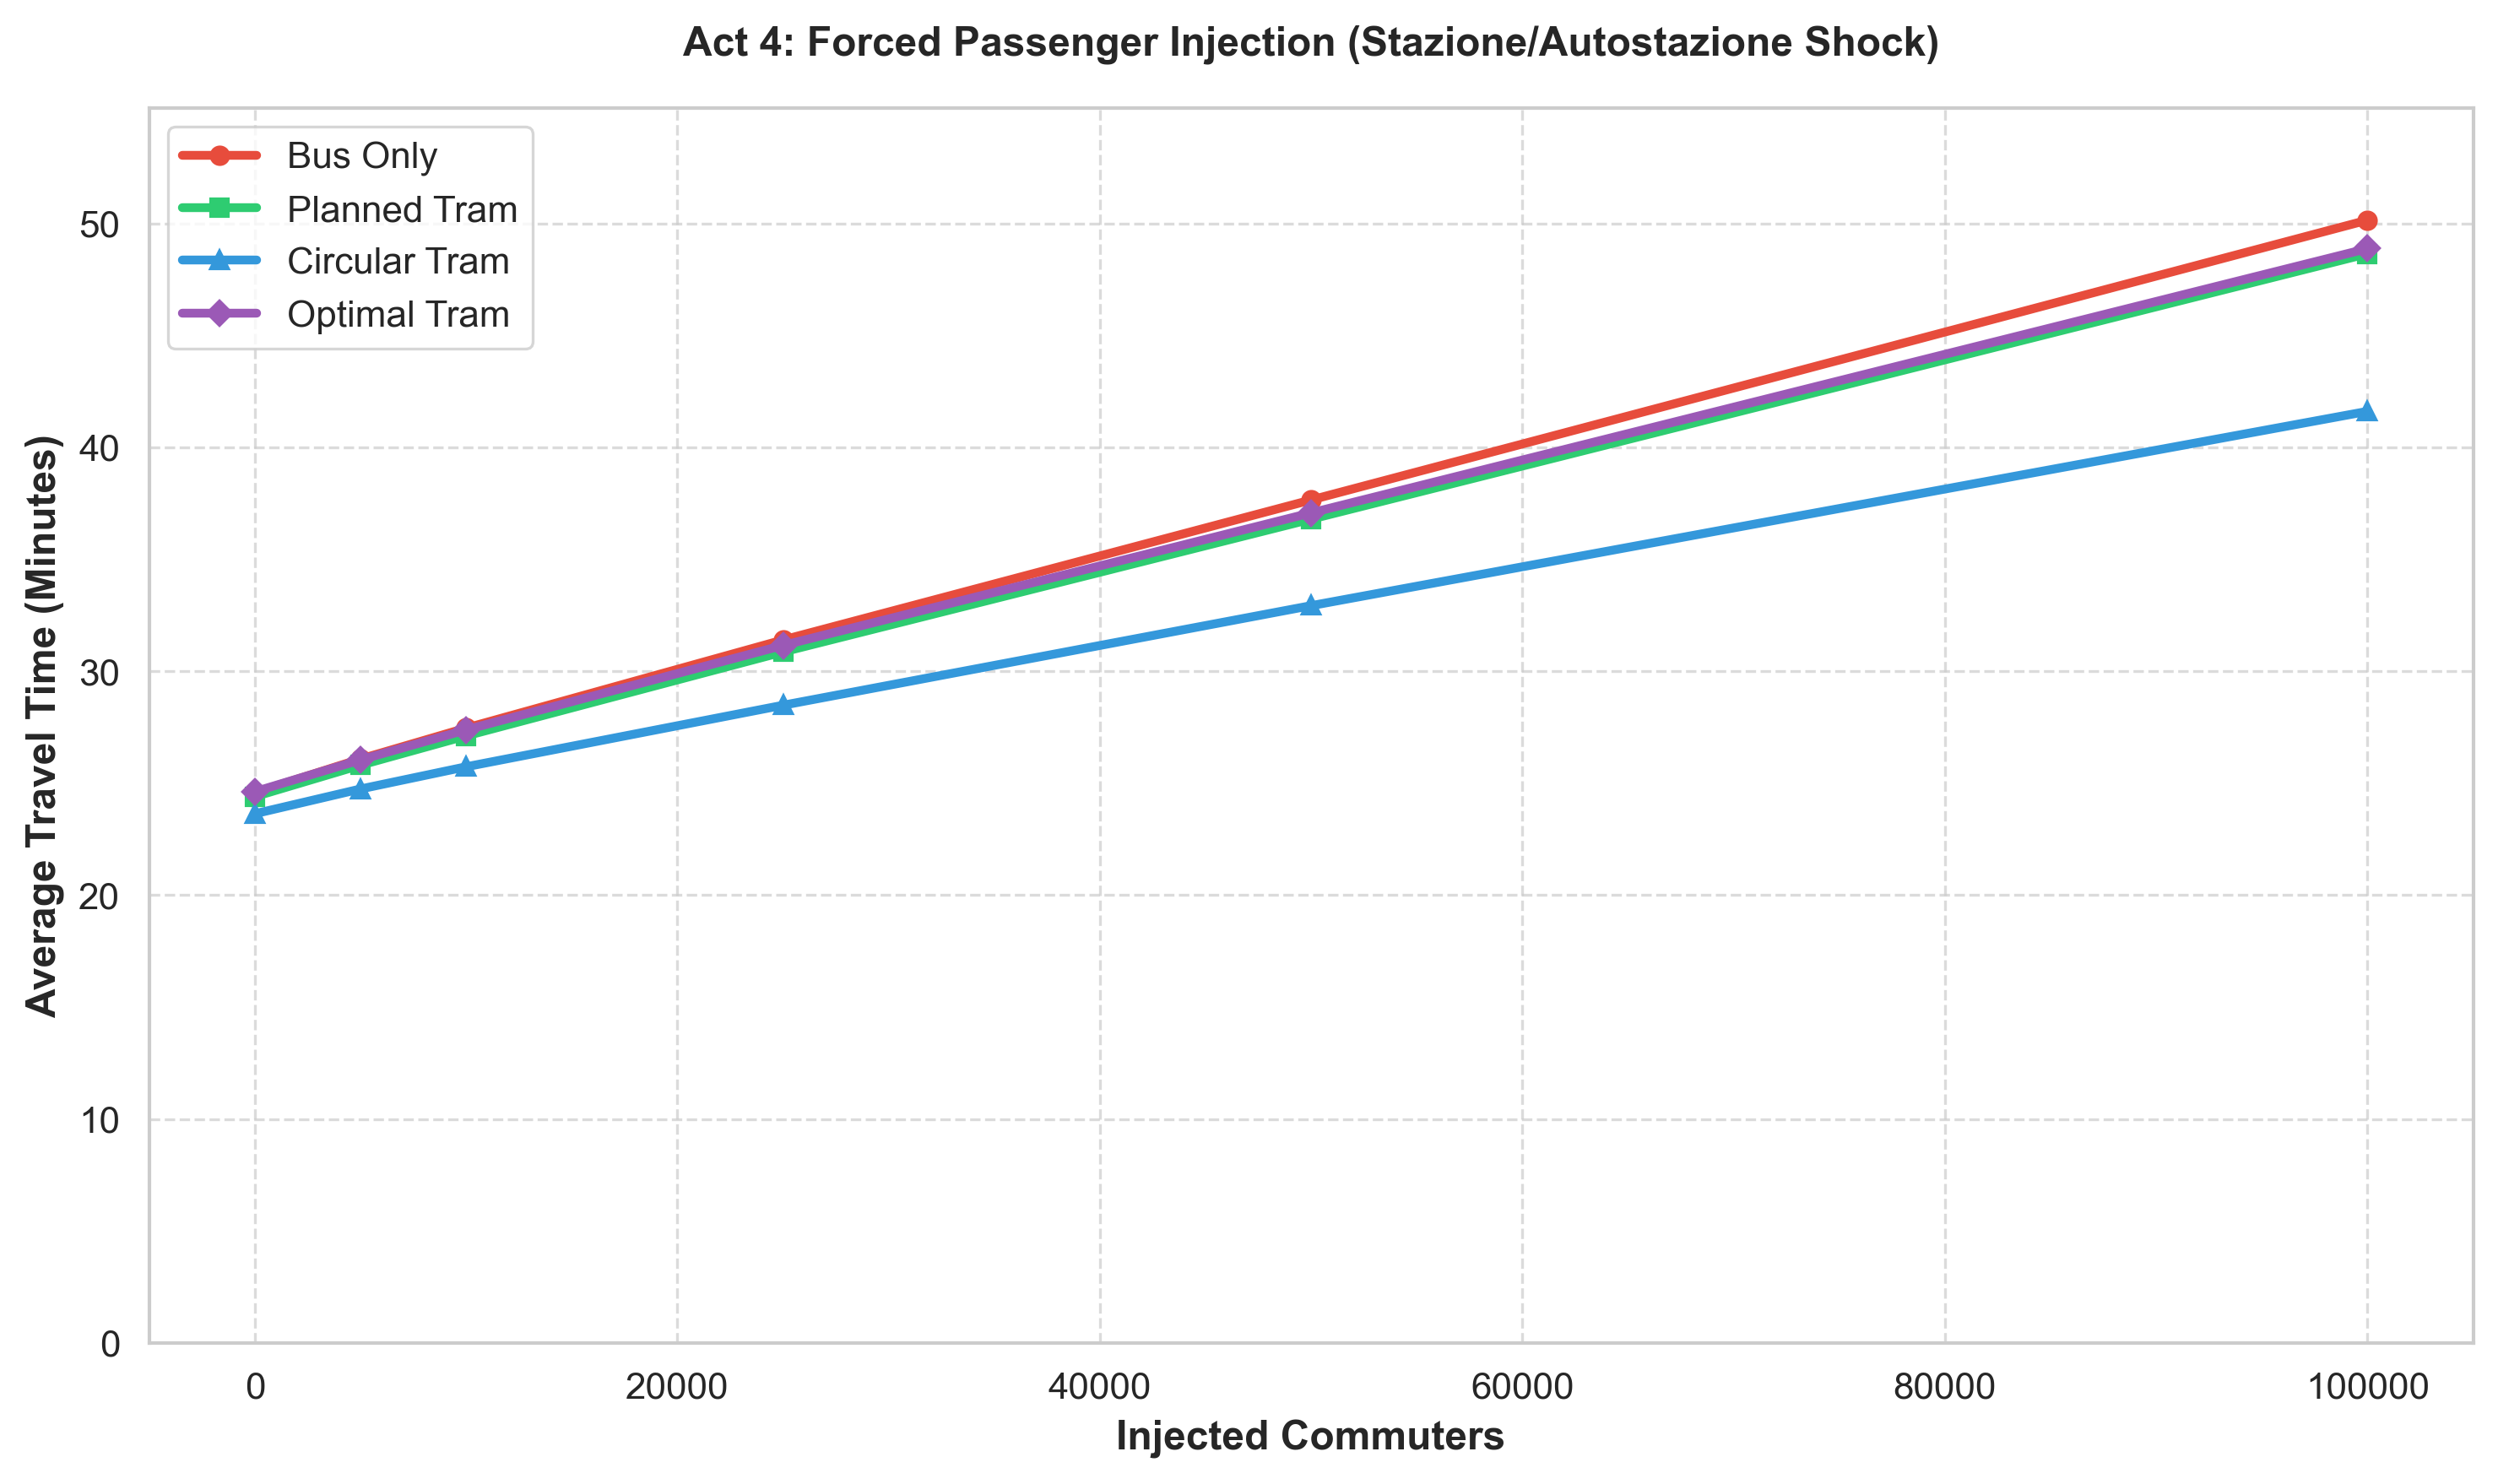
\includegraphics[width=\textwidth]{figures/bologna/bologna_forced_injection_shock.png}
        \caption{Average travel time from the injection hubs as a function of the injected commuter volume.}
        \label{fig:forced_injection}
    \end{minipage}
\end{figure}

We simulated the simultaneous arrival of up to 100,000 commuters by inflating the dynamic dwell time on all edges incident to the two hubs, and measured the average shortest-path travel time from the hubs to every other stop (Figure~\ref{fig:forced_injection}). Table~\ref{tab:injection_shock_results} reports the resulting averages in minutes.

\begin{table}[H]
    \centering
    \caption{Average Travel Times (minutes) under Forced Hub Passenger Injection}
    \label{tab:injection_shock_results}
    \begin{tabular}{ccccc}
        \toprule
        Injected Passengers & Bus Only & Planned Tram & Circular Tram & Optimal Tram \\
        \midrule
        0 & 24.58 & 24.40 & 23.64 & 23.39 \\
        5,000 & 26.08 & 25.80 & 24.74 & 24.82 \\
        10,000 & 27.46 & 27.11 & 25.73 & 26.15 \\
        25,000 & 31.40 & 30.86 & 28.48 & 29.89 \\
        50,000 & 37.65 & 36.80 & 32.93 & 35.80 \\
        100,000 & 50.15 & 48.66 & 41.61 & 47.61 \\
        \bottomrule
    \end{tabular}
\end{table}

Under a massive commuter shock of 100,000 passengers:
\begin{itemize}
    \item The Bus Only, Planned Tram, and Optimal Tram networks experience extreme congestion, with average travel times roughly doubling (from about 23--25 minutes to about 48--50 minutes).
    \item The Circular Tram mitigates the congestion, maintaining an average travel time of \textbf{41.61 minutes} --- a saving of \textbf{7.05 minutes} ($14.5\%$) over the Planned Tram layout.
    \item \textbf{Physical interpretation}: Since Stazione Centrale and Autostazione lie directly on the historic ring road, upgrading the circular corridor (Lines 32/33) into a fast tramway lets commuters disperse immediately clockwise and counter-clockwise without entering the congested core. In contrast, the radial Planned Tram lines (Red and Green) and the Optimal Tram layout route passengers through the historic centre, which becomes a bottleneck under high commuter volumes. Circular bypass corridors are therefore essential to absorb passenger shocks originating at central inter-modal hubs.
\end{itemize}

\section{Conclusion}
\label{conclusion}

The analysis shows that transit networks are highly sensitive to spatial chokepoints and localized demand shocks. Radial layouts, such as the Planned Tram's Red/Green lines and our Optimal Tram design, are effective at speeding up travel across the municipal area, but they funnel passengers through the city centre and are therefore vulnerable to localized passenger injections at the major hubs. Circular corridors, such as the Circular Tram, act as vital orbital loops that route flows around the historic core. A resilient transit strategy for Bologna should therefore balance high-capacity radial lines with circular bypass corridors, absorbing commuter shocks and preventing systemic congestion collapse.

\section{Critique}
\label{critique}

Several limitations of the present pipeline should be acknowledged:
\begin{enumerate}
    \item \textbf{Static Demand Proxy}: Resident population mapped to stops is used as a proxy for demand, which does not capture actual origin--destination (O--D) passenger matrices. A more advanced approach would ingest real ticketing (smart card) data to weight nodes by observed passenger volumes.
    \item \textbf{Local-Optimum Bias}: The greedy tramway optimizer grows lines step-by-step from seed nodes and can be trapped in local optima. Metaheuristics such as evolutionary algorithms or simulated annealing could yield better global designs.
    \item \textbf{No Explicit Transfer Friction}: Bus--tram interchanges within the $30\text{ m}$ snapping radius are merged into single nodes, so line changes incur no waiting or inconvenience penalty in the model. In reality, transfers impose both waiting times (dependent on heterogeneous line headways) and a cognitive cost; a multilayer formulation with explicit transfer edges would capture this friction.
\end{enumerate}

Despite these limitations, the study demonstrates the value of Network Science for evaluating urban transport interventions, suggesting that the Bologna tramway can substantially improve city-wide mobility --- especially if radial lines are complemented by an orbital bypass corridor.

\bibliographystyle{plain}
\bibliography{references}
\end{document}
